% ============================================================
% PREPRINT STYLE CONFIGURATION
% Matches visual style of "ABIDES-MARL" (2511.02016v1)
%============================================================
\documentclass[11pt, a4paper]{article}
\usepackage{float}
% 1. TYPOGRAPHY: Times New Roman for text and math
\usepackage[T1]{fontenc}
\usepackage{newtxtext}       % Times text font
\usepackage{newtxmath}       % Times math font
\usepackage[final]{microtype} % Professional kerning

% 2. PAGE GEOMETRY
\usepackage[left=1in, right=1in, top=1in, bottom=1in]{geometry}
\setlength{\parindent}{1.5em} % Standard paragraph indentation
\setlength{\parskip}{0pt}     % Standard paragraph spacing

% 3. HEADER AND FOOTER
\pagestyle{plain}

% 4. TITLE BLOCK & AFFILIATIONS
\usepackage{authblk}
\renewcommand\Affilfont{\itshape\small} % Affiliations in italics
\makeatletter
\renewcommand{\maketitle}{
    \begin{center}
        {\LARGE \bfseries \@title \par}
        \vspace{1.0em}
        {\large \@author \par}
        \vspace{0.5em}
        {\itshape \@date}
    \end{center}
    \vspace{1.0em}
}
\makeatother

% 5. ABSTRACT & KEYWORDS STYLING
\usepackage{abstract}
\renewcommand{\abstractname}{}    % Hide "Abstract" title for cleaner look
\renewcommand{\absnamepos}{empty}

% 6. CITATIONS & LINKS
\usepackage[authoryear, round]{natbib}
\bibliographystyle{plainnat}

% 7. MATH & ALGORITHMS
% Avoid \openbox clash (some fonts/packages define it before amsthm)
\let\openbox\relax
\usepackage{amsmath,amsthm,mathtools,bm}
\usepackage{aliascnt}

% Links, then cleveref (after amsthm) for theorem-like references.
\usepackage[colorlinks=true, allcolors=blue]{hyperref}
\usepackage{xurl}
\urlstyle{same}
\usepackage{placeins}
\usepackage[capitalize,nameinlink]{cleveref}
\usepackage{siunitx}
\sisetup{detect-all}
\usepackage{booktabs}
\usepackage{graphicx}
\usepackage{listings}
\usepackage{algorithm}
\usepackage{algpseudocode}
\usepackage{orcidlink}

% 8. MACROS & THEOREMS
\theoremstyle{plain}
\newtheorem{theorem}{Theorem}

\newaliascnt{lemma}{theorem}
\newtheorem{lemma}[lemma]{Lemma}
\aliascntresetthe{lemma}

\newaliascnt{proposition}{theorem}
\newtheorem{proposition}[proposition]{Proposition}
\aliascntresetthe{proposition}

\newaliascnt{corollary}{theorem}
\newtheorem{corollary}[corollary]{Corollary}
\aliascntresetthe{corollary}

\theoremstyle{definition}
\newaliascnt{definition}{theorem}
\newtheorem{definition}[definition]{Definition}
\aliascntresetthe{definition}

\theoremstyle{remark}
\newaliascnt{remark}{theorem}
\newtheorem{remark}[remark]{Remark}
\aliascntresetthe{remark}

% hyperref \autoref names for theorem-like environments sharing a counter.
\providecommand*{\theoremautorefname}{Theorem}
\providecommand*{\lemmaautorefname}{Lemma}
\providecommand*{\propositionautorefname}{Proposition}
\providecommand*{\corollaryautorefname}{Corollary}
\providecommand*{\definitionautorefname}{Definition}
\providecommand*{\remarkautorefname}{Remark}

% Explicit cleveref names for shared theorem counter environments.
\crefname{theorem}{Theorem}{Theorems}
\Crefname{theorem}{Theorem}{Theorems}
\crefname{lemma}{Lemma}{Lemmas}
\Crefname{lemma}{Lemma}{Lemmas}
\crefname{proposition}{Proposition}{Propositions}
\Crefname{proposition}{Proposition}{Propositions}
\crefname{corollary}{Corollary}{Corollaries}
\Crefname{corollary}{Corollary}{Corollaries}
\crefname{definition}{Definition}{Definitions}
\Crefname{definition}{Definition}{Definitions}
\crefname{remark}{Remark}{Remarks}
\Crefname{remark}{Remark}{Remarks}

\newcommand{\R}{\mathbb{R}}
\newcommand{\E}{\mathbb{E}}
\newcommand{\Var}{\operatorname{Var}}
\newcommand{\Cov}{\operatorname{Cov}}
\newcommand{\ind}{\mathbb{I}}

% Custom keyword command matching target style
\newcommand{\keywords}[1]{\vspace{1em}\noindent\textbf{Keywords:} #1}

% ============================================================
% DOCUMENT METADATA
% ============================================================
\title{Robust Discrete Pricing Optimization via Multiple-Choice Knapsack Reductions}
\author[1]{Zi Yuan Eric Shao}
\affil[1]{Department of Mathematics, ETH Zürich, \texttt{ershao@student.ethz.ch}}
\date{March 2026}


% ============================================================
\begin{document}
\maketitle

\begin{abstract}
We study a discrete portfolio pricing problem that selects one price per product from a finite menu under margin and fairness constraints. To account for demand uncertainty, we incorporate a budgeted robust formulation that controls conservatism while remaining computationally tractable. By reducing the problem to a Multiple-Choice Knapsack Problem (MCKP), we identify structural properties of the LP relaxation---in particular, upper-hull filtering and greedy filling over hull segments---that yield an exact solution method for the LP relaxation of the fixed-parameter subproblems. For the resulting fixed-parameter subproblems, we show that the integrality gap is bounded additively by a single-item hull jump, and that the corresponding relative gap decays as \(O(1/n)\) under standard boundedness and linear-growth assumptions. Numerical experiments on synthetic portfolios and a stylized retail case study with economically calibrated parameters are consistent with these bounds and indicate that robust margin protection can be achieved with less than 1\% nominal revenue loss on the instances tested.
\end{abstract}

\keywords{Discrete Optimization; Robust Optimization; Pricing; Knapsack Problem}

\section{Introduction and Reduction}\label{sec:intro}
We consider a pricing optimization problem where a decision maker must set prices for a collection of items in order to maximize overall value (e.g., profit or revenue), subject to two key constraints. First, the portfolio must achieve at least a prescribed margin level, so that overall profitability remains acceptable. Second, each individual price must stay sufficiently close to a given reference or ``fair'' price, reflecting regulatory, actuarial, or market considerations. Problems of this type arise repeatedly in practice, for instance in insurance tariff setting, retail and e-commerce pricing, or energy and telecom tariffs, whenever large price menus must be adjusted under margin and fairness constraints.

Two modeling choices deserve brief justification. We work with \emph{discrete} price menus because many applied settings (e.g., insurance tariffs, retail shelf prices with psychological endings, and standardized energy contracts) restrict the decision maker to a finite set of admissible price points, and continuous relaxations can therefore produce infeasible prices. We also impose the margin requirement as a \emph{ratio} constraint $N(\bm{x})/D(\bm{x}) \geq \Delta$ rather than an additive floor $N(\bm{x}) - D(\bm{x}) \geq b$. The ratio form is scale-invariant and matches standard profitability metrics such as loss ratio and gross-margin percentage.
\paragraph{Contributions.}
Our contributions are threefold.
\begin{enumerate}
\item[(i)] We formulate a discrete portfolio pricing problem with ratio-based margin and fairness constraints and show that it reduces \emph{exactly} to a Multiple-Choice Knapsack Problem (MCKP). While the MCKP is classical, the reduction from constrained pricing with ratio margins, fairness bands, and weighted demand provides a direct bridge between pricing practice and combinatorial optimization theory.

\item[(ii)] We introduce a $\Gamma$-budget robust extension of this MCKP and prove that the coupled robust constraint admits a \emph{parametric dual decomposition} (\Cref{thm:parametric}) that reduces the problem to a one-dimensional enumeration over a finite breakpoint set (\Cref{prop:theta_candidates_discrete_clean}). This yields a specialized structure-exploiting algorithmic framework for the $\Gamma$-budget robust MCKP that avoids relying on a generic MILP reformulation inside the main solution loop.

\item[(iii)] We establish that the integrality gap of each fixed-$\theta$ subproblem is bounded additively by a single item's maximum hull-value jump $\Delta V^{\theta}_{\max}$ (\Cref{prop:igap_additive_theta_clean}), yielding a relative gap of \(O(1/n)\) for large portfolios (\Cref{cor:igap_relative_theta_clean}). Numerical experiments on synthetic and economically calibrated instances are consistent with these bounds and indicate that robust margin protection costs less than $1\%$ of nominal revenue on the instances tested.
\end{enumerate}
The LP relaxation analysis in \Cref{sec:structure} (\Cref{thm:master_greedy}) consolidates known MCKP relaxation properties \citep{Dyer1984,Pisinger1995} and is re-proved in a self-contained way in our notation. The main novelty lies in contributions (ii) and~(iii) and in the end-to-end pipeline connecting the pricing formulation to a specialized robust optimization procedure built around hull-based LP structure.

\subsection{Problem Formulation}
\noindent Mathematically we have the following discrete problem. For each class $i\in\{1,\dots,n\}$, we choose one price level $x_i \in \mathcal X_i=\{x_{i,1},\dots,x_{i,m}\}.$ We are given parameters for each class $i$: reference price $a_i>0$, weight exposure $\omega_i$, nominal demand $\hat{g}_i:\mathcal{X}_i\to \R_{\geq0}$ (monotone decreasing on the admissible range; e.g.\ piecewise-linear or iso-elastic), relative tolerance $\sigma_i$, and a margin target parameter $\Delta>0$.
We assume the demand functions $\hat{g}_i$ depend only on the own-price $x_i$ and not on other items' prices, which is appropriate when cross-product substitution is negligible (see \Cref{sec:conclusion} for extensions).

\noindent \textbf{Define}:
\[
N(\bm{x}) \coloneqq \sum_{i=1}^n \omega_i\,x_i\,\hat{g}_i(x_i),\qquad
D(\bm{x}) \coloneqq \sum_{i=1}^n \omega_i\,a_i\,\hat{g}_i(x_i)>0,\qquad
S(\bm{x}) \coloneqq N(\bm{x})-\Delta \cdot D(\bm{x})\ .
\]
\textbf{Optimization Problem}:
\begin{align}
\max_{\bm{x}}\quad & N(\bm{x})=\sum_{i=1}^n \omega_i x_i \hat{g}_i(x_i),\\
\text{s.\,t.}\quad &
\frac{N(\bm{x})}{D(\bm{x})}\ \ge\ \Delta\ \ \Leftrightarrow\ \ S(\bm{x})\ge0,\\
&
\frac{|x_i - a_i|}{a_i} \le \sigma_i \iff x_{i}\in [(1-\sigma_{i} )a_{i},\  (1+\sigma_{i} )a_{i}] \quad (\forall i).
\end{align}
The second constraint can be easily mitigated by defining the admissible menu
\[
I_{i}:=\left[ \left( 1-\sigma_{i} \right) a_{i},\  \left( 1+\sigma_{i} \right) a_{i} \right], \qquad
\mathcal X_i^{\mathrm{ad}} := \mathcal X_i \cap I_i \neq \emptyset,\qquad i=1,\dots,n,
\]
and henceforth restrict all decisions to $x_i\in \mathcal X_i^{\mathrm{ad}}$.


\subsection{Reduction to MCKP}\label{par:MCKP}
For a formal introduction to the classical 0--1 Knapsack problem and the standard MCKP definition, we refer to \Cref{app:background}.
Introduce binary selection variables $z_{ij}\in\{0,1\}$ indicating the choice $x_i=x_{i,j}$. For each option $x_{i,j}\in\mathcal X_i$, define
\begin{align}
    v_{ij} & \coloneqq \omega_i\,x_{i,j}\,\hat{g}_i(x_{i,j}), \\
    d_{ij} & \coloneqq \omega_i\,a_i\,\hat{g}_i(x_{i,j}), \\
    s_{ij} & \coloneqq v_{ij}-\Delta\,d_{ij}.
\end{align}
Let $J_i^{\mathrm{ad}}:=\{j\in\{1,\dots,m\}: x_{i,j}\in \mathcal X_i^{\mathrm{ad}}\}$ denote the admissible indices. Then
\[
N(\bm x)=\sum_{i=1}^n\sum_{j\in J_i^{\mathrm{ad}}} v_{ij}z_{ij},
\qquad
S(\bm x)=\sum_{i=1}^n\sum_{j\in J_i^{\mathrm{ad}}} s_{ij}z_{ij},
\qquad
\sum_{j\in J_i^{\mathrm{ad}}} z_{ij}=1 \ \ (\forall i).
\]
To obtain a single knapsack constraint with nonnegative costs, apply a baseline--slack transformation. For each $i$ choose a baseline option
\begin{align*}
    j^*(i) & \in \operatorname*{arg\,max}_{j\in J_i^{\mathrm{ad}}} s_{ij}, \\
    S_{\text{max}} & \coloneqq \sum_{i=1}^n s_{i\,j^*(i)}, \\
    c_{ij} & \coloneqq s_{i\,j^*(i)}-s_{ij}\ \ (\ge 0)\qquad (j\in J_i^{\mathrm{ad}}).
\end{align*}
Then
\[
\sum_{i=1}^n\sum_{j\in J_i^{\mathrm{ad}}} s_{ij}z_{ij}
\;=\;
\sum_{i=1}^n s_{i\,j^*(i)}
\;-\;
\sum_{i=1}^n\sum_{j\in J_i^{\mathrm{ad}}} c_{ij}z_{ij}
\;=\;
S_{\text{max}}-\sum_{i=1}^n\sum_{j\in J_i^{\mathrm{ad}}} c_{ij}z_{ij}.
\]
Hence the ratio constraint $S(\bm{x})\ge 0$ is equivalent to the knapsack inequality
\[
\sum_{i=1}^n\sum_{j\in J_i^{\mathrm{ad}}} c_{ij}\,z_{ij} \;\le\; S_{\text{max}}.
\]
The pricing problem is therefore exactly the multiple-choice knapsack problem (MCKP)
\begin{align}
    \max \quad & \sum_{i=1}^n \sum_{j\in J_i^{\mathrm{ad}}} v_{ij}\,z_{ij} \\
    \text{s.t.}\quad & \sum_{i=1}^n \sum_{j\in J_i^{\mathrm{ad}}} c_{ij}\,z_{ij} \;\le\; S_{\text{max}}, \\
    & \sum_{j\in J_i^{\mathrm{ad}}} z_{ij}=1 \quad (i=1,\dots,n), \\
    & z_{ij}\in\{0,1\}\quad (\forall i,\ j\in J_i^{\mathrm{ad}}).
\end{align}


\section{Related Work}
\label{sec:related_work}

\paragraph{MCKP foundations.}
The Multiple-Choice Knapsack Problem (MCKP) is a classical discrete optimization model in which exactly one option is selected from each of $n$
groups under a knapsack constraint. Early work established NP-hardness and developed exact methods based on branch-and-bound and dominance
preprocessing; see, e.g., \citet{Nauss1978,Ibaraki1978,Sinha1979}. A key structural feature is the near-integrality of the LP relaxation:
there exists an optimal LP solution in which all but at most one group choose a single option, while one group (at most) is mixed between
two options \citep{Dyer1984}. This LP structure underpins many exact and heuristic schemes and is closely related to convex-hull and ``core''
ideas used in practical solvers \citep{Pisinger1995,Kellerer2004}.

\paragraph{Extensions and uncertainty.}
Motivated by applications in large-scale pricing and resource allocation, recent work has considered generalizations such as setup decisions
and additional side constraints, where decomposition and matheuristics become effective (e.g., \citealp{Boukhari2023,Boukhari2024}). In
parallel, uncertainty in demand and cost parameters has renewed interest in approaches beyond purely stochastic models, which often require
distributional information that is unavailable or unreliable. Robust Optimization (RO) provides an attractive alternative \citep{BenTal1999},
and the budgeted uncertainty model of \citet{BertsimasSim2004} ($\Gamma$-robustness) controls the trade-off between conservatism and performance
while preserving tractability properties for many linear problems. Recent applications have illustrated the value of this approach in multi-product
pricing under interval uncertainties \citep{Hamzeei2022}.

\paragraph{Gap addressed in this paper.}
For knapsack-type problems, exact and combinatorial algorithms for robust variants are well studied in the single-choice setting
(e.g., \citealp{Monaci2013}). In contrast, the multiple-choice setting with $\Gamma$-budget coupling has received comparatively less attention in terms of specialized, structure-exploiting algorithms. The formulation of \citet{Caserta2019} relies
on a generic MILP reformulation of the robust constraints together with kernel-search-style matheuristics, without exploiting the MCKP's
upper-hull LP structure. Extensions such as locally budgeted uncertainty further enrich modeling flexibility \citep{Goerigk2021}, but these
formulations are typically validated through general-purpose solvers rather than structure-specific algorithms. The present paper exploits the
convex-hull LP structure of the MCKP \emph{within} a $\Gamma$-budget robust framework, yielding a specialized algorithmic approach with
provable integrality-gap bounds. The pricing reduction of \Cref{sec:intro} provides the applied motivation; the
structural and algorithmic results (\Cref{sec:structure,sec:algorithm}) apply to any MCKP with $\Gamma$-budget uncertainty in the capacity
constraint, independent of the pricing interpretation.
% ============================================================
% SECTION: STRUCTURAL ANALYSIS
% ============================================================
\section{Robust Pricing under Demand Uncertainty}\label{sec:robust}

In the formulation presented in \Cref{sec:intro}, the demand response $\hat{g}_i(x_i)$ is treated as a deterministic function of price even though demand estimates are subject to statistical error. To mitigate this risk, we introduce a \textbf{Budgeted Robust} framework in which the true demand $\tilde{g}_i(x_i)$ resides in an uncertainty set $\mathcal U$ and the margin constraint must hold for \textit{all} realizations in that set. We then seek a price vector $\bm{x}$ that maximizes nominal revenue subject to this worst-case feasibility requirement.

\subsection{Uncertainty Model}
We assume the realized demand lies within a symmetric interval around the nominal value:
\begin{equation}
    \tilde{g}_i(x_i) \in [\hat{g}_i(x_i) - \delta_i(x_i), \hat{g}_i(x_i) + \delta_i(x_i)],
\end{equation}
where $\delta_i(x_i) \ge 0$ is a variability parameter (e.g., derived from the standard error of the demand estimation). We assume $\delta_i(x_i)\le \hat g_i(x_i)$ on $\mathcal X_i^{\mathrm{ad}}$, so demand remains nonnegative under uncertainty.

To avoid overly conservative solutions—such as those arising from box uncertainty where every product realizes its worst-case simultaneously—we adopt the ``Budget of Uncertainty'' approach proposed by \citet{BertsimasSim2004}. We define an integer budget $\Gamma \in \{0,1,\dots,n\}$, representing the maximum number of products that can simultaneously deviate to their worst-case limits.

\begin{definition}[Uncertainty Set]
Let $\xi_i \in [-1, 1]$ be the scaled deviation for item $i$. For a fixed price vector $x$, we define the uncertainty set $\mathcal{U}^\Gamma$ as:
\begin{equation}
    \mathcal{U}^\Gamma(\bm{x}) = \left\{ \tilde{g}(\bm{x}) \in \mathbb{R}^n \;\bigg|\; \tilde{g}_i(x_i) = \hat{g}_i(x_i) + \xi_i \delta_i(x_i), \quad \sum_{i=1}^n |\xi_i| \le \Gamma, \quad |\xi_i| \le 1 \quad \forall i \right\}.
\end{equation}
\end{definition}

\subsection{The Robust Counterpart}
The robust margin constraint requires $S(\bm{x}) \ge 0$ for all $\tilde{g} \in \mathcal{U}^\Gamma(\bm{x})$. Substituting the definitions of $N(\bm{x})$ and $D(\bm{x})$, this condition is equivalent to:
\begin{equation}\label{eq:robust_raw}
    \min_{\tilde{g} \in \mathcal{U}^\Gamma(\bm{x})} \sum_{i=1}^n \omega_i \tilde{g}_i(x_i) (x_i - \Delta a_i) \ge 0.
\end{equation}
Let $s_i(x_i)=\omega_{i} \left( x_{i}-\Delta a_{i} \right) \hat{g}_{i} \left( x_{i} \right)$ and $t_i(x_i):=\omega_i(x_i-\Delta a_i)\,\delta_i(x_i).$ The robust constraint can be rewritten as:
\begin{equation}\label{eq:robust_st}
    \sum_{i=1}^n s_i(x_i) + \min_{\xi : \sum |\xi_i| \le \Gamma, |\xi_i| \le 1} \sum_{i=1}^n t_i(x_i) \xi_i \ge 0.
\end{equation}
The minimization term represents the worst-case deviation permitted by the budget. Since the objective is linear in $\xi_i$, the minimum is achieved when $\xi_i$ takes values on the boundary of its domain to oppose the sign of $\omega_i(x_i-\Delta a_i)$. This worst-case behavior leads to the following exact formulation:

\begin{theorem}[Robust Counterpart Formulation]\label{thm:robust}
Let $\Gamma \in \{0,1,\dots,n\}$ be an integer. Define
\[
\beta(\bm{x},\Gamma)
\ :=\
\sum_{k=1}^{\Gamma} \ |t|_{(k)}(\bm{x}),
\]
where $|t|_{(1)}(\bm{x}) \ge \cdots \ge |t|_{(n)}(\bm{x})$ denotes the nonincreasing ordering of the numbers
$\big\{|t_i(x_i)|\big\}_{i=1}^n$. We adopt the convention that $\beta(\bm{x},0)=0$.
Then the robust optimization problem is equivalent to
\begin{align}
    \max_{\bm{x}} \quad & \sum_{i=1}^n \omega_i x_i \hat{g}_i(x_i) \\
    \text{s.t.} \quad 
    & \sum_{i=1}^n s_i(x_i) - \beta(\bm{x}, \Gamma) \ge 0, \label{eq:robust_final}\\
    & x_i \in [(1-\sigma_i)a_i,(1+\sigma_i)a_i]\cap \mathcal X_i \qquad (\forall i). \nonumber
\end{align}
\end{theorem}

\begin{proof}
Fix $\bm{x}$ and consider the inner minimization in \eqref{eq:robust_st}:
\[
V(\bm{x})
=
\min_{\substack{\sum_{i=1}^n|\xi_i|\le \Gamma\\ |\xi_i|\le 1}}
\ \sum_{i=1}^n t_i(x_i)\,\xi_i .
\]
By feasibility and symmetry of the constraints, for any feasible $\bm{\xi}$ we may flip signs coordinatewise so that
$\operatorname{sgn}(\xi_i)=-\operatorname{sgn}(t_i(x_i))$ whenever $\xi_i\neq 0$, without violating
$\sum_i|\xi_i|\le \Gamma$ or $|\xi_i|\le 1$. This is valid because $|\xi_i|$ is invariant under sign changes, so neither the budget constraint
nor the box constraint is affected. Hence
\[
V(\bm{x})
=
-\max_{\substack{\sum_{i=1}^n y_i \le \Gamma\\ 0\le y_i \le 1}}
\ \sum_{i=1}^n |t_i(x_i)|\,y_i ,
\qquad\text{where } y_i:=|\xi_i|.
\]
The maximization problem above is a linear program. Since $\Gamma$ is an integer, it admits an optimal extreme point solution
with $y_i\in\{0,1\}$ for all $i$ and $\sum_i y_i\le \Gamma$.
Therefore an optimal solution sets $y_i=1$ for the $\Gamma$ indices with largest coefficients $|t_i(x_i)|$ and $y_i=0$ otherwise, giving
\[
V(\bm{x})
=
-\sum_{k=1}^{\Gamma} |t|_{(k)}(\bm{x})
=
-\beta(\bm{x},\Gamma).
\]
Substituting this into \eqref{eq:robust_st} yields \eqref{eq:robust_final}.
\end{proof}

\section{Structural Analysis and Greedy Optimality}\label{sec:structure}

The $\Gamma$-budget penalty $\beta(\bm{x},\Gamma)$ couples items and breaks separability, which is a main source of computational difficulty
in robust discrete pricing. Even without robustness, the reduced problem is NP-hard because it is an MCKP. The key structural observation is
that the LP relaxation remains efficiently solvable: each item's discrete menu induces an upper hull in the cost--value plane, and the global
LP reduces to greedy filling over hull segments. The sequel derives this hull-greedy LP structure and connects it to the robust model through
the parametric decomposition used in \Cref{sec:algorithm}.

\subsection{Upper-hull geometry of the LP relaxation}\label{subsec:hull_lp}
Fix an item $i$ and consider its admissible discrete options $x_{i,j}\in\mathcal X_i^{\mathrm{ad}}$ from \Cref{sec:intro}.
Each option induces a point $(c_{ij},v_{ij})$ in the cost--value plane, and we write
\[
\mathcal P_i \;:=\;\{(c_{ij},v_{ij}) : x_{i,j}\in\mathcal X_i^{\mathrm{ad}}\}\subset\mathbb R^2.
\]
In the LP relaxation, the constraints $\sum_j z_{ij}=1$ and $z_{ij}\ge 0$ allow fractional mixing across options; equivalently, item $i$
may realize any aggregate point $(c_i,v_i)\in\operatorname{conv}(\mathcal P_i)$. Since the objective maximizes value for a given resource
usage, only points on the \emph{upper hull} of $\operatorname{conv}(\mathcal P_i)$ can be optimal. This motivates
\emph{upper-hull filtering}: we replace $\mathcal P_i$ by the ordered vertex sequence $\mathcal H_i$ of the upper hull of
$\operatorname{conv}(\mathcal P_i)$, thereby discarding dominated menu points without changing the LP optimum.

\begin{remark}(Economic intuition)\label{rem:diminishing_returns}
In many pricing portfolios, spending additional margin slack yields progressively smaller revenue gains, suggesting a concave
``efficiency frontier''. The analysis below does not assume such concavity on the raw discrete menus: concavity arises automatically after
passing to the upper hull of $\operatorname{conv}(\mathcal P_i)$.
\end{remark}

Assume the LP is feasible, equivalently $C \ge \sum_i \min_j c_{ij}$ (and in particular $C \ge \sum_i c^H_{i,1}$).
\begin{remark}[Relation to prior work]\label{rem:prior_hull}
The properties collected in \Cref{thm:master_greedy} are individually standard in the MCKP literature; see \citet{Dyer1984}, \citet{Pisinger1995}, and \citet[Chapter~11]{Kellerer2004}. We re-prove them in unified form because our notation differs from these sources and the segment parameterization is used directly in \Cref{sec:algorithm}. Readers familiar with the classical MCKP LP structure may skip ahead to the Robust Constraint Structure subsection without loss of continuity.
\end{remark}
\begin{theorem}[Hull reduction and greedy optimality for the LP relaxation]\label{thm:master_greedy}
Consider the LP relaxation of the Multiple-Choice Knapsack Problem (MCKP):
\begin{align}\label{eq:lp_mckp_master}
\max_{\bm{z}} \quad & \sum_{i=1}^n\sum_{j=1}^m v_{ij}\,z_{ij}\\
\text{s.t.}\quad & \sum_{i=1}^n\sum_{j=1}^m c_{ij}\,z_{ij}\le C,\nonumber\\
& \sum_{j=1}^m z_{ij}=1 \quad (i=1,\dots,n),\nonumber\\
& z_{ij}\ge 0 \quad (\forall i,j).\nonumber
\end{align}
For each item $i$, define the point set $\mathcal P_i:=\{(c_{ij},v_{ij}) : j=1,\dots,m\}\subset\mathbb R^2$.
Let $\mathcal H_i=\{(c^H_{i,1},v^H_{i,1}),\allowbreak\dots,\allowbreak(c^H_{i,p_i},v^H_{i,p_i})\}$ denote the vertices of the \emph{upper hull}
of $\operatorname{conv}(\mathcal P_i)$, ordered so that $c^H_{i,1}<\cdots<c^H_{i,p_i}$.
For $k=1,\dots,p_i-1$ define the hull segment lengths and slopes
\[
\Delta c^H_{i,k}:=c^H_{i,k+1}-c^H_{i,k}>0,
\qquad
\rho^H_{i,k}:=\frac{v^H_{i,k+1}-v^H_{i,k}}{c^H_{i,k+1}-c^H_{i,k}}.
\]

Then the following statements hold.

\begin{enumerate}
\item[(i)] (\textbf{Upper-hull sufficiency / two-adjacent-vertices mixing.})
There exists an optimal solution to \eqref{eq:lp_mckp_master} such that for each $i$,
the induced aggregate point $(c_i,v_i):=\big(\sum_j c_{ij}z_{ij},\sum_j v_{ij}z_{ij}\big)$ lies on the upper hull of
$\operatorname{conv}(\mathcal P_i)$, and hence can be represented as a convex combination of at most two \emph{adjacent} hull vertices
$(c^H_{i,k},v^H_{i,k})$ and $(c^H_{i,k+1},v^H_{i,k+1})$ for some $k$.

\item[(ii)] (\textbf{Reduction to continuous knapsack over hull segments.})
The LP \eqref{eq:lp_mckp_master} is equivalent to the continuous knapsack problem
\begin{align}\label{eq:cont_knap_master}
\max_{\bm{\ell}} \quad & \sum_{i=1}^n\sum_{k=1}^{p_i-1}\rho^H_{i,k}\,\ell_{i,k}\\
\text{s.t.}\quad & \sum_{i=1}^n\sum_{k=1}^{p_i-1}\ell_{i,k}\ \le\ C-\sum_{i=1}^n c^H_{i,1},\nonumber\\
& 0\le \ell_{i,k}\le \Delta c^H_{i,k}\qquad(\forall i,k),\nonumber
\end{align}
where $\ell_{i,k}$ denotes the amount of capacity allocated to hull segment $k$ of item $i$.

\item[(iii)] (\textbf{Greedy optimality for the LP relaxation.})
Let $\bm{\ell}^\star$ be obtained by filling segment variables $\ell_{i,k}$ in nonincreasing order of densities $\rho^H_{i,k}$,
each up to its upper bound $\Delta c^H_{i,k}$, with at most one final fractional fill to meet the capacity constraint.
Then $\bm{\ell}^\star$ induces an optimal solution to \eqref{eq:cont_knap_master} and hence an optimal solution to the LP relaxation
\eqref{eq:lp_mckp_master}. In particular, there exists an optimal LP solution in which at most one item is mixed fractionally
(i.e.\ across two adjacent hull vertices); all other items select a single hull vertex.

\item[(iv)] (\textbf{Special case: incremental greedy on the raw chain.})
Suppose for every $i$ the raw point chain $\{(c_{i,j},v_{i,j})\}_{j=1}^m$ satisfies
$c_{i,1}<\cdots<c_{i,m}$ and lie on the upper hull of $\operatorname{conv}(\mathcal P_i)$.
Thus they coincide with the hull vertices.
Then the greedy rule in (iii) reduces to the \emph{incremental greedy algorithm} on adjacent increments
$\rho_{i,j}=(v_{i,j}-v_{i,j-1})/(c_{i,j}-c_{i,j-1})$.
\end{enumerate}
\end{theorem}

\begin{proof}
Steps 1--3 (convex-hull reformulation, restriction to the upper hull, and segment-length parameterization) follow standard arguments adapted to our notation; we defer them to \Cref{app:thm2_steps} for completeness.

\textbf{Proof of (iii).}
Problem \eqref{eq:cont_knap_master} is a continuous knapsack (fractional) problem with items indexed by pairs $(i,k)$,
value density $\rho^H_{i,k}$ and capacity upper bound $\Delta c^H_{i,k}$.
A standard exchange argument shows that an optimal solution is obtained by filling variables in nonincreasing order of $\rho^H_{i,k}$:
take two variables $(i,k)$ and $(i',k')$ with $\rho^H_{i,k}>\rho^H_{i',k'}$. If $0<\ell_{i',k'}<\Delta c^H_{i',k'}$ while
$\ell_{i,k}<\Delta c^H_{i,k}$, then shifting an infinitesimal amount $\varepsilon$ of capacity from $\ell_{i',k'}$ to $\ell_{i,k}$
increases the objective by $\varepsilon(\rho^H_{i,k}-\rho^H_{i',k'})>0$ while preserving feasibility, contradicting optimality.
Thus, in any optimum, all higher-density variables are saturated before any lower-density variable is positive, implying the greedy fill rule
is optimal and that at most one variable can be fractional at termination. This proves (iii).

\textbf{Proof of (iv).}
If for each $i$ the raw chain coincides with the hull vertices, i.e.\
$\mathcal H_i=\{(c_{i,j},v_{i,j})\}_{j=1}^m$,
then the hull segments are exactly the adjacent increments $(j-1)\to j$ and $\rho^H_{i,k}$ equals $\rho_{i,j}$.
Therefore the greedy rule in (iii) reduces to selecting adjacent upgrades in descending order of $\rho_{i,j}$, which is precisely the
incremental greedy algorithm. \qedhere
\end{proof}

\subsection{Robust Constraint Structure}
\subsubsection{Box Uncertainty (\texorpdfstring{$\Gamma=n$}{Gamma=n}): Separability}
We first address the structural impact of robustness in the limiting case of \textbf{Box Uncertainty}, i.e.\ when the budget equals the number of items ($\Gamma=n$). In this regime, every item may simultaneously deviate to its worst-case limit.

Recall the robust margin constraint in the form \eqref{eq:robust_st}:
\[
\sum_{i=1}^n s_i(x_i) + \min_{\substack{\sum_{i=1}^n|\xi_i|\le \Gamma\\|\xi_i|\le 1}} \ \sum_{i=1}^n t_i(x_i)\,\xi_i \ \ge\ 0,
\qquad
s_i(x)=\omega_i(x-\Delta a_i)\hat g_i(x),\quad
t_i(x)=\omega_i(x-\Delta a_i)\delta_i(x).
\]
For $\Gamma=n$, the budget constraint $\sum_i|\xi_i|\le n$ is redundant given $|\xi_i|\le 1$, and the inner minimum is attained by choosing
$\xi_i=-\operatorname{sgn}(t_i(x_i))$, yielding
\begin{equation}\label{eq:box_constraint}
\sum_{i=1}^n s_i(x_i)\;-\;\sum_{i=1}^n |t_i(x_i)|\ \ge\ 0.
\end{equation}
Hence the box-robust pricing problem can be written as
\begin{align}
    \max_{\bm{x}} \quad & \sum_{i=1}^n v_i(x_i)
\qquad\text{where } v_i(x):=\omega_i\,x\,\hat g_i(x), \label{eq:box_problem}\\
    \text{s.t.} \quad & \sum_{i=1}^n\Big(s_i(x_i)-|t_i(x_i)|\Big)\ \ge\ 0, \nonumber\\
    & x_i \in \mathcal X_i\cap[(1-\sigma_i)a_i,(1+\sigma_i)a_i]\qquad(\forall i). \nonumber
\end{align}
In contrast to the coupled case $\Gamma<n$, the penalty in \eqref{eq:box_constraint} is additive and therefore separable across items.


\subsubsection{Coupled Uncertainty (\texorpdfstring{$\Gamma<n$}{Gamma<n}): Parametric Decomposition}
For the coupled case $\Gamma<n$, items interact through the shared uncertainty budget.
By \Cref{thm:robust}, the robust margin constraint is equivalent to
\begin{equation}\label{eq:robust_coupled_raw}
\sum_{i=1}^n s_i(x_i)\;-\;\beta(\bm{x},\Gamma)\ \ge\ 0,
\end{equation}
where $\beta(\bm{x},\Gamma)=\sum_{k=1}^\Gamma |t|_{(k)}(\bm{x})$ is the sum of the $\Gamma$ largest values of $\{|t_i(x_i)|\}_{i=1}^n$.
While this characterization is explicit, direct optimization over $\beta(\bm{x},\Gamma)$ is difficult because it couples all items
through a sorting operation. We resolve this by observing that $\beta(\bm{x},\Gamma)$ admits a dual scalar representation:
\begin{equation}\label{eq:inner_knap}
\beta(\bm{x},\Gamma)
=\max_{\bm{\xi}}\left\{\sum_{i=1}^n |t_i(x_i)|\,\xi_i \ \middle|\ \sum_{i=1}^n \xi_i\le \Gamma,\ 0\le \xi_i\le 1\ \forall i\right\}.
\end{equation}
\begin{theorem}[Parametric decomposition of the coupled $\Gamma$-budget penalty]\label{thm:parametric}
For every $\bm{x}$, the penalty $\beta(\bm{x},\Gamma)$ in \eqref{eq:inner_knap} admits the dual representation
\begin{equation}\label{eq:psi_dual}
\beta(\bm{x},\Gamma)
=\min_{\theta\ge 0}\Bigg\{\Gamma\theta+\sum_{i=1}^n \max\big\{0,\ |t_i(x_i)|-\theta\big\}\Bigg\}.
\end{equation}
Consequently, the robust margin constraint \eqref{eq:robust_coupled_raw} holds if and only if there exists $\theta\ge 0$ such that
\begin{equation}\label{eq:dual_robust_clean}
\sum_{i=1}^n\Big(s_i(x_i)-\max\big\{0,\ |t_i(x_i)|-\theta\big\}\Big)\ \ge\ \Gamma\theta.
\end{equation}
For any fixed $\theta\ge 0$, the left-hand side of \eqref{eq:dual_robust_clean} is separable across items.
\end{theorem}
\begin{proof}
Fix $\bm{x}$. Problem \eqref{eq:inner_knap} is a feasible and bounded linear program over a nonempty compact polytope.
Its dual is
\[
\min_{\theta\ge 0,\ \bm{\pi}\ge 0}\ \Gamma\theta+\sum_{i=1}^n \pi_i
\quad\text{s.t.}\quad
\theta+\pi_i\ge |t_i(x_i)|\ \ (\forall i).
\]
Strong duality yields equality of primal and dual optimal values. For any fixed $\theta\ge 0$, the minimal feasible choice is
$\pi_i=\max\{0,\ |t_i(x_i)|-\theta\}$, which gives \eqref{eq:psi_dual}. Substituting \eqref{eq:psi_dual} into
\eqref{eq:robust_coupled_raw} yields \eqref{eq:dual_robust_clean}.
\end{proof}
% ============================================================
% SECTION: A Robust Hull-Greedy Algorithm for the Discrete Problem
% ============================================================
\section{A Robust Hull-Greedy Algorithm for the Discrete Problem}\label{sec:algorithm}

We develop a method for the \emph{discrete} $\Gamma$-budget robust pricing problem. After the reduction in \Cref{sec:intro}, the
problem is an MCKP and remains NP-hard, so we target exact robust-feasibility certification together with explicit performance guarantees relative to LP benchmarks.
The algorithm is driven by two structural results: the one-dimensional parametric reformulation of the coupled robust constraint
(\Cref{thm:parametric}) and the exact hull-greedy solution of the fixed-parameter LP relaxation (\Cref{thm:master_greedy}).

\subsection{Exact robust feasibility via a scalar parameter}\label{subsec:theta}

For each admissible option $x_{i,j}\in\mathcal X_i^{\mathrm{ad}}$, define
\[
v_{ij}:=\omega_i\,x_{i,j}\,\hat g_i(x_{i,j}),\qquad
s_{ij}:=\omega_i\,(x_{i,j}-\Delta a_i)\,\hat g_i(x_{i,j}),\qquad
t_{ij}:=\omega_i\,(x_{i,j}-\Delta a_i)\,\delta_i(x_{i,j}).
\]
By \Cref{thm:parametric}, the robust margin constraint is equivalent to the existence of $\theta\ge 0$ such that
\begin{equation}\label{eq:theta_feas_clean}
\sum_{i=1}^n\Big(s_i(x_i)-\max\{0,\ |t_i(x_i)|-\theta\}\Big)\ \ge\ \Gamma\theta.
\end{equation}
For fixed $\theta\ge 0$, introduce the per-option $\theta$-modified contributions
\begin{equation}\label{eq:s_theta_def_clean}
s^\theta_{ij}\;:=\;s_{ij}-\max\{0,\ |t_{ij}|-\theta\}.
\end{equation}
Then \eqref{eq:theta_feas_clean} becomes the separable inequality
\begin{equation}\label{eq:theta_margin_clean}
\sum_{i=1}^n s^\theta_{i,\,j(i)}\ \ge\ \Gamma\theta,
\qquad j(i)\in\{1,\dots,m\}\ \text{chosen for each }i.
\end{equation}
\noindent where $j(i)$ denotes the index of the option selected for item $i$.

\begin{proposition}[Finite candidate set for \texorpdfstring{$\theta$}{theta}]\label{prop:theta_candidates_discrete_clean}
Let
\[
\mathcal B\;:=\;\{0\}\ \cup\ \{|t_{ij}|:\ i=1,\dots,n,\ x_{i,j}\in\mathcal X_i^{\mathrm{ad}}\}.
\]
If the discrete robust problem is feasible, then there exists an optimal solution $(\bm x^\star,\theta^\star)$ with $\theta^\star\in\mathcal B$.
\end{proposition}

\begin{proof}
Fix a discrete $\bm x$. Define
\[
f_{\bm x}(\theta)
:=\sum_{i=1}^n\Big(s_i(x_i)-\max\{0,\ |t_i(x_i)|-\theta\}\Big)-\Gamma\theta.
\]
Then $f_{\bm x}$ is concave piecewise-affine in $\theta$, with breakpoints contained in $\{0\}\cup\{|t_i(x_i)|\}_{i=1}^n$.
If $f_{\bm x}(\theta_0)\ge 0$ for some $\theta_0\ge 0$, let $[\theta_L,\theta_U]$ be the maximal interval containing $\theta_0$ on which
$f_{\bm x}$ is affine (so $\theta_L,\theta_U$ are breakpoints, with $\theta_L=\theta_U=\theta_0$ possible). Since $f_{\bm x}$ is affine on
$[\theta_L,\theta_U]$, at least one endpoint satisfies $f_{\bm x}(\theta)\ge 0$ (because a non-negative affine function on an interval attains its minimum at an endpoint), and thus feasibility for fixed $\bm x$ can always be certified
by some breakpoint $\theta\in\{0\}\cup\{|t_i(x_i)|\}_{i=1}^n$. Because each $|t_i(x_i)|$ equals $|t_{i,j(i)}|$ for some admissible option,
every such value belongs to~$\mathcal B$. Since this argument holds for every discrete $\bm x$ individually, the joint optimum
$(\bm x^\star,\theta^\star)$ is covered by enumerating $\theta\in\mathcal B$ and, for each fixed~$\theta$, optimizing over discrete~$\bm x$---which is precisely the structure exploited by Algorithm~\ref{alg:robust_hull_greedy}.
\end{proof}

\subsection{Fixed-\texorpdfstring{$\theta$}{theta} reformulation as an MCKP}\label{subsec:theta_mckp}

Fix $\theta\in\mathcal B$. Convert \eqref{eq:theta_margin_clean} into a knapsack inequality with nonnegative costs via a baseline--slack
transformation. For each item $i$, choose
\[
j^\theta(i)\in\operatorname*{arg\,max}_{j}\ s^\theta_{ij},\qquad
S^\theta_{\max}:=\sum_{i=1}^n s^\theta_{i,\,j^\theta(i)},\qquad
c^\theta_{ij}:=s^\theta_{i,\,j^\theta(i)}-s^\theta_{ij}\ \ (\ge 0).
\]
Then \eqref{eq:theta_margin_clean} is equivalent to
\begin{equation}\label{eq:theta_knapsack_clean}
\sum_{i=1}^n c^\theta_{i,\,j(i)}\ \le\ C^\theta,
\qquad
C^\theta:=S^\theta_{\max}-\Gamma\theta.
\end{equation}
Thus, for fixed $\theta$, robust-feasible discrete pricing is exactly the MCKP
\begin{equation}\label{eq:mckp_theta_clean}
\max \ \sum_{i=1}^n v_{i,\,j(i)}
\quad\text{s.t.}\quad
\sum_{i=1}^n c^\theta_{i,\,j(i)}\le C^\theta,
\quad
x_{i,j(i)}\in\mathcal X_i^{\mathrm{ad}}\ \ (\forall i).
\end{equation}

\subsection{Upper-hull filtering and an exact LP solver for fixed \texorpdfstring{$\theta$}{theta}}\label{subsec:hull_theta}

Fix $\theta\in\mathcal B$ with $C^\theta\ge 0$. Item $i$ induces the point set
\[
\mathcal P_i^\theta:=\{(c^\theta_{ij},v_{ij}) : x_{i,j}\in\mathcal X_i^{\mathrm{ad}}\}\subset\mathbb R^2.
\]
Before computing the hull, apply a standard preprocessing step: (a) if multiple points share the same cost $c$, keep only the one with
largest value $v$; (b) remove dominated points (if $c\le c'$ and $v\ge v'$, discard $(c',v')$). This does not change the upper hull.
Apply \emph{upper-hull filtering} by replacing $\mathcal P_i^\theta$ with the ordered vertex sequence
\[
\mathcal H_i^\theta=\{(c^{H,\theta}_{i,1},v^{H,\theta}_{i,1}),\dots,(c^{H,\theta}_{i,p_i},v^{H,\theta}_{i,p_i})\}
\]
of the upper hull of $\operatorname{conv}(\mathcal P_i^\theta)$ (ordered by increasing $c$). Since $\mathcal H_i^\theta$ consists of
vertices of $\operatorname{conv}(\mathcal P_i^\theta)$, each hull vertex is one of the original menu points $(c^\theta_{ij},v_{ij})$ and
therefore corresponds to a discrete option.
Define hull segment lengths and slopes
\[
\Delta c^{H,\theta}_{i,k}:=c^{H,\theta}_{i,k+1}-c^{H,\theta}_{i,k}>0,\qquad
\rho^{H,\theta}_{i,k}:=\frac{v^{H,\theta}_{i,k+1}-v^{H,\theta}_{i,k}}{\Delta c^{H,\theta}_{i,k}}
\quad (k=1,\dots,p_i-1).
\]
By \Cref{thm:master_greedy}, the LP relaxation of \eqref{eq:mckp_theta_clean} is solved \emph{exactly} by greedily filling hull segments in
nonincreasing order of $\rho^{H,\theta}_{i,k}$. Moreover, there exists an optimal LP solution in which at most one item is fractional (mixed
between two adjacent hull vertices).

\paragraph{Exact robust-feasibility certificate (final check).}\label{par:cert}
For any discrete price vector $\bm x$, robust feasibility can be certified directly by
\begin{equation}\label{eq:certify_alg}
\sum_{i=1}^n s_i(x_i)\;-\;\beta(\bm{x},\Gamma)\ \ge\ 0,
\qquad
\beta(\bm{x},\Gamma)=\sum_{k=1}^{\Gamma}|t|_{(k)}(\bm{x}),
\end{equation}
where $t_i(x)=\omega_i(x-\Delta a_i)\delta_i(x)$ and $|t|_{(1)}(\bm{x})\ge\cdots\ge|t|_{(n)}(\bm{x})$ are the sorted magnitudes.

\subsection{Discrete recovery: one-item rounding with optional repair}\label{subsec:rounding}

Let $\bm z^{\mathrm{LP}}(\theta)$ be an optimal LP solution produced by the hull-greedy procedure in \Cref{subsec:hull_theta}.
If no item is fractional, it is already discrete. Otherwise, exactly one item $i^\star$ is mixed between two adjacent hull vertices
$(c^{H,\theta}_{i^\star,k},v^{H,\theta}_{i^\star,k})$ and $(c^{H,\theta}_{i^\star,k+1},v^{H,\theta}_{i^\star,k+1})$.

\paragraph{Default choice (feasibility-preserving round-down).}
Rounding $i^\star$ \emph{down} to the adjacent vertex with smaller knapsack cost $c^\theta$ weakly decreases total cost and thus preserves
\eqref{eq:theta_knapsack_clean}; all other items remain unchanged. This yields a feasible discrete solution $\bm x^{\downarrow}(\theta)$.

\paragraph{Optional improvement (round-up + repair).}
In practice, rounding down can lose a larger single-item value jump than necessary. As an optional refinement, also consider rounding
$i^\star$ \emph{up} to the higher vertex, obtaining $\bm x^{\uparrow}(\theta)$, which may violate \eqref{eq:theta_knapsack_clean} by some
excess cost $\Delta C>0$. If $\Delta C>0$, restore feasibility by a \emph{repair} step that performs discrete \emph{downgrades} on other
items along their hull chains: repeatedly select a downgrade that reduces knapsack cost by at least a small amount while minimizing loss of
objective, specifically by selecting the downgrade $(i, k \to k{-}1)$ along item $i$'s hull chain that minimizes the ratio
$(v^{H,\theta}_{i,k}-v^{H,\theta}_{i,k-1})/(c^{H,\theta}_{i,k}-c^{H,\theta}_{i,k-1})$ among items with remaining downgrade capacity, until total cost is $\le C^\theta$. Since downgrades weakly decrease total cost, feasibility
is restored after finitely many steps. Finally, keep the better of the two feasible candidates,
\[
\bm x(\theta)\in\arg\max\{N(\bm x^{\downarrow}(\theta)),\ N(\bm x^{\uparrow\!\to\!\mathrm{repair}}(\theta))\}.
\]
This refinement is heuristic but feasibility-preserving. All theoretical guarantees (Propositions~\ref{prop:rg_additive_theta} and~\ref{prop:igap_additive_theta_clean}) apply to the round-down solution $\bm x^{\downarrow}(\theta)$ alone; the optional round-up-and-repair and completion steps can only improve the objective and are not required for the stated bounds.

\paragraph{Feasibility-preserving completion.}
While capacity remains, apply discrete \emph{upgrades} along each item's hull chain (adjacent hull vertices) in decreasing order of slope
among upgrades that fit. This can only improve the objective and preserves \eqref{eq:theta_knapsack_clean}.

\subsection{Complete algorithm and guarantees}\label{subsec:rg_full}

We enumerate $\theta\in\mathcal B$ (which is sufficient by \Cref{prop:theta_candidates_discrete_clean}), solve the corresponding LP
relaxation exactly by hull-greedy, and recover a discrete feasible solution by one-item rounding (optionally with repair/completion); see
Algorithm~\ref{alg:robust_hull_greedy}.

\begin{proposition}[Additive performance bound (per fixed $\theta$)]\label{prop:rg_additive_theta}
Fix $\theta\in\mathcal B$ with $C^\theta\ge 0$. Let $\mathrm{OPT}_{\mathrm{LP}}(\theta)$ and $\mathrm{OPT}_{\mathrm{IP}}(\theta)$ denote the
optimal objective values of the LP relaxation of \eqref{eq:mckp_theta_clean} and of \eqref{eq:mckp_theta_clean}, respectively.
Let $\bm x(\theta)$ be the rounded solution produced by Algorithm~\ref{alg:robust_hull_greedy} (before optional post-processing). Then
\[
\mathrm{OPT}_{\mathrm{LP}}(\theta)-N(\bm x(\theta))\ \le\ \Delta V_{\max}^\theta,
\qquad\text{and hence}\qquad
\mathrm{OPT}_{\mathrm{IP}}(\theta)-N(\bm x(\theta))\ \le\ \Delta V_{\max}^\theta,
\]
where $\Delta V_{\max}^\theta$ is defined in \Cref{subsec:igap}.
\end{proposition}

\begin{proof}
By \Cref{thm:master_greedy}(iii), there exists an optimal LP solution mixing at most one item between two adjacent hull vertices.
Rounding down that item (to the adjacent vertex with smaller $c^\theta$) preserves feasibility and decreases the objective by at most the
corresponding adjacent value jump, bounded by $\Delta V_{\max}^\theta$. The second inequality follows from
$\mathrm{OPT}_{\mathrm{LP}}(\theta)\ge \mathrm{OPT}_{\mathrm{IP}}(\theta)$.
\end{proof}

\begin{algorithm}[H]
\footnotesize
\caption{Robust hull-greedy with $\theta$-enumeration and discrete recovery}\label{alg:robust_hull_greedy}
\begin{algorithmic}[1]
\State \textbf{Input:} admissible menus $\{\mathcal X_i^{\mathrm{ad}}\}$, data $(v_{ij},s_{ij},t_{ij})$, budget $\Gamma$.
\State Form $\mathcal B=\{0\}\cup\{|t_{ij}|:\ x_{i,j}\in\mathcal X_i^{\mathrm{ad}}\}$, deduplicate, and sort increasingly.
\State $\textsc{BestVal}\leftarrow -\infty$, $\textsc{BestSol}\leftarrow \emptyset$.
\For{$\theta\in\mathcal B$}
    \State Compute $s^\theta_{ij}$ via \eqref{eq:s_theta_def_clean}.
    \State Choose $j^\theta(i)\in\arg\max_j s^\theta_{ij}$ and set $c^\theta_{ij}=s^\theta_{i,\,j^\theta(i)}-s^\theta_{ij}$.
    \State $C^\theta\leftarrow \sum_{i=1}^n s^\theta_{i\,j^\theta(i)}-\Gamma\theta$. \If{$C^\theta<0$} \textbf{continue}. \EndIf
    \For{$i=1,\dots,n$}
        \State Build $\mathcal P_i^\theta=\{(c^\theta_{ij},v_{ij})\}_j$.
        \State Preprocess $\mathcal P_i^\theta$: merge equal costs (keep max $v$), then remove dominated points.
        \State Compute the upper hull $\mathcal H_i^\theta$ and the slopes $\rho^{H,\theta}_{i,k}$ and lengths $\Delta c^{H,\theta}_{i,k}$.
    \EndFor
    \State Solve the LP relaxation of \eqref{eq:mckp_theta_clean} exactly via hull-greedy over $\rho^{H,\theta}_{i,k}$.
    \State Recover a discrete solution $\bm x(\theta)$ via \Cref{subsec:rounding} (round-down; optionally round-up+repair; optionally complete).
    \State Compute $N(\bm x(\theta))=\sum_{i=1}^n \omega_i\,x_i(\theta)\,\hat g_i(x_i(\theta))$.
    \State Compute the exact robust certificate $Z(\bm x(\theta)):=\sum_i s_i(x_i(\theta))-\beta(\bm x(\theta),\Gamma)$ as in \eqref{eq:certify_alg}.
    \If{$Z(\bm x(\theta))<0$} \textbf{continue}. \EndIf
    \If{$N(\bm x(\theta))>\textsc{BestVal}$}
        \State $\textsc{BestVal}\leftarrow N(\bm x(\theta))$; $\textsc{BestSol}\leftarrow (\theta,\bm x(\theta))$.
    \EndIf
\EndFor
\If{$\textsc{BestSol}=\emptyset$}
    \State \textbf{Output:} \textsc{Infeasible} (no $\theta\in\mathcal B$ yields $C^\theta\ge 0$ and a feasible selection).
\Else
    \State \textbf{Output:} $\textsc{BestSol}$.
\EndIf
\end{algorithmic}
\end{algorithm}

\paragraph{Practical note on $\theta$ enumeration.}
The set $\mathcal B$ can be as large as $|\mathcal B|\le nm+1$, but in practice the search can be reduced substantially by restricting
candidates to breakpoints induced by undominated options (after preprocessing). Moreover, \eqref{eq:s_theta_def_clean} implies
\[
s^\theta_{ij}=
\begin{cases}
s_{ij}, & \theta\ge |t_{ij}|,\\
s_{ij}-|t_{ij}|+\theta, & \theta<|t_{ij}|,
\end{cases}
\]
so $s^\theta_{ij}$ is piecewise-affine in $\theta$ with breakpoints at $|t_{ij}|$. Consequently, per-item maximizers $j^\theta(i)\in\arg\max_j
s^\theta_{ij}$ can only change at such breakpoints, suggesting sweep-style implementations that update per-item baselines incrementally rather
than recomputing from scratch. Regardless of the search strategy, the certificate \eqref{eq:certify_alg} provides an exact final check.

% ============================================================
% INTEGRALITY GAP (BENCHMARKING JUSTIFICATION)
% ============================================================
\subsection{Integrality gap and its asymptotic irrelevance}\label{subsec:igap}

For benchmarking, we compare discrete solutions against the LP relaxation of \eqref{eq:mckp_theta_clean}. For fixed $\theta$,
$\mathrm{OPT}_{\mathrm{LP}}(\theta)\ge \mathrm{OPT}_{\mathrm{IP}}(\theta)$, and the gap is controlled by a \emph{single} item.

\medskip
\noindent\textbf{Setup (fixed $\theta$).}
Fix $\theta\in\mathcal B$ with $C^\theta\ge 0$. For each item $i$, let
\[
\mathcal P_i^\theta:=\{(c^\theta_{ij},v_{ij}) : x_{i,j}\in\mathcal X_i^{\mathrm{ad}}\}\subset\mathbb R^2,
\]
and let $\mathcal H_i^\theta=\{(c^{H,\theta}_{i,1},v^{H,\theta}_{i,1}),\dots,(c^{H,\theta}_{i,p_i},v^{H,\theta}_{i,p_i})\}$
be the upper-hull vertex sequence of $\operatorname{conv}(\mathcal P_i^\theta)$, ordered by strictly increasing cost
$c^{H,\theta}_{i,1}<\cdots<c^{H,\theta}_{i,p_i}$.
Define the maximal adjacent hull jump
\[
\Delta V_{\max}^\theta
:=\max_{i}\ \max_{k=1,\dots,p_i-1}\big(v^{H,\theta}_{i,k+1}-v^{H,\theta}_{i,k}\big)\ \ge\ 0,
\]
with the convention $\max_{k\in\emptyset}(\cdot)=0$ when $p_i=1$.

\begin{proposition}[Additive integrality-gap bound]\label{prop:igap_additive_theta_clean}
For every fixed $\theta\in\mathcal B$ with $C^\theta\ge 0$,
\[
0\ \le\ \mathrm{OPT}_{\mathrm{LP}}(\theta)-\mathrm{OPT}_{\mathrm{IP}}(\theta)\ \le\ \Delta V_{\max}^\theta .
\]
\end{proposition}

\begin{proof}
The lower bound is immediate since the LP relaxation enlarges the feasible set. For the upper bound, by
\Cref{thm:master_greedy}(i)--(iii) there exists an optimal LP solution in which at most one item $i^\star$ is fractional, and if fractional
it mixes between two \emph{adjacent} hull vertices $(c^{H,\theta}_{i^\star,k},v^{H,\theta}_{i^\star,k})$ and
$(c^{H,\theta}_{i^\star,k+1},v^{H,\theta}_{i^\star,k+1})$ for some $k$. If no item is fractional, the LP solution is integral and the gap
is $0$.

Otherwise, the fractional point has the form
\[
(c_{i^\star},v_{i^\star})
=(1-\alpha)(c^{H,\theta}_{i^\star,k},v^{H,\theta}_{i^\star,k})+\alpha(c^{H,\theta}_{i^\star,k+1},v^{H,\theta}_{i^\star,k+1}),
\qquad \alpha\in(0,1).
\]
Round $i^\star$ down to the cheaper endpoint $(c^{H,\theta}_{i^\star,k},v^{H,\theta}_{i^\star,k})$ and keep all other items unchanged.
Total knapsack cost weakly decreases, hence feasibility is preserved. The objective decreases by at most the adjacent jump
$v^{H,\theta}_{i^\star,k+1}-v^{H,\theta}_{i^\star,k}$, because $v_{i^\star}$ lies between the endpoint values. Thus
\[
\mathrm{OPT}_{\mathrm{LP}}(\theta)-\mathrm{OPT}_{\mathrm{IP}}(\theta)
\ \le\ v^{H,\theta}_{i^\star,k+1}-v^{H,\theta}_{i^\star,k}
\ \le\ \Delta V_{\max}^\theta,
\]
as claimed.
\end{proof}

\begin{corollary}[Relative gap decays as \(O(1/n)\)]\label{cor:igap_relative_theta_clean}
Assume there exist constants $\overline V<\infty$ and $c>0$ such that for all $\theta\in\mathcal B$,
\[
\Delta V_{\max}^\theta\le \overline V,
\qquad
\mathrm{OPT}_{\mathrm{LP}}(\theta)\ge c\,n.
\]
Then for all $\theta\in\mathcal B$,
\[
0\ \le\
\frac{\mathrm{OPT}_{\mathrm{LP}}(\theta)-\mathrm{OPT}_{\mathrm{IP}}(\theta)}{\mathrm{OPT}_{\mathrm{LP}}(\theta)}
\ \le\
\frac{\overline V}{c\,n}
\ =\ O\!\left(\frac{1}{n}\right).
\]
\end{corollary}

\begin{proof}
By \Cref{prop:igap_additive_theta_clean},
$\mathrm{OPT}_{\mathrm{LP}}(\theta)-\mathrm{OPT}_{\mathrm{IP}}(\theta)\le \Delta V_{\max}^\theta\le \overline V$.
Divide by $\mathrm{OPT}_{\mathrm{LP}}(\theta)\ge c\,n>0$.
\end{proof}

\paragraph{When do \texorpdfstring{$\overline V$}{Vbar} and $c$ exist? (Sufficient conditions)}
The assumptions $\Delta V_{\max}^\theta\le \overline V$ and $\mathrm{OPT}_{\mathrm{LP}}(\theta)\ge c\,n$ express two standard regularities:
(i) per-item value scales do not blow up, and (ii) the portfolio has nondegenerate average value. A convenient sufficient set is:

\medskip
\noindent\textbf{(A) Uniform bounded values.}
If there exists $M_v<\infty$ such that $0\le v_{ij}\le M_v$ for all items $i$, all admissible options $j\in J_i^{\mathrm{ad}}$, and all
$\theta\in\mathcal B$, then $\Delta V_{\max}^\theta\le M_v$ for all $\theta$ (take $\overline V:=M_v$), since hull vertices are menu points
and differences of two numbers in $[0,M_v]$ are at most $M_v$.
A concrete sufficient condition for such an $M_v$ is
$\sup_i\omega_i<\infty$, $\sup_{i,j}x_{i,j}<\infty$, and $\sup_{i,j}\hat g_i(x_{i,j})<\infty$, because then
$v_{ij}=\omega_i x_{i,j}\hat g_i(x_{i,j})$ is uniformly bounded.

\medskip
\noindent\textbf{(B) Uniform positive value in a feasible baseline.}
If there exists $m_v>0$ such that for each item $i$ there is an admissible option $j\in J_i^{\mathrm{ad}}$ that is feasible for the fixed-$\theta$
knapsack constraint and satisfies $v_{ij}\ge m_v$ (independently of $n$), then there is a feasible integer solution with value at least
$m_v n$, hence $\mathrm{OPT}_{\mathrm{LP}}(\theta)\ge \mathrm{OPT}_{\mathrm{IP}}(\theta)\ge m_v n$ (take $c:=m_v$).
In pricing applications this is typically ensured by assuming each item has a ``safe'' admissible baseline price that preserves the margin
constraint with slack, and exposures/demand at that baseline are bounded away from zero.

\paragraph{Practical implication.}
Under (A)--(B), the absolute LP--IP gap is controlled by a single-item jump while $\mathrm{OPT}_{\mathrm{LP}}(\theta)=\Omega(n)$, so the
relative gap vanishes as $n\to\infty$. Hence the LP relaxation provides an essentially tight benchmark for large portfolios.

% ============================================================
% SECTION: NUMERICAL RESULTS
% ============================================================
\section{Numerical Results}\label{sec:numerics}

We empirically examine three consequences of the structural analysis developed in
\Cref{sec:structure,sec:algorithm}:
(i) the rounding loss is bounded by a single hull jump and the relative gap decays as \(O(1/n)\)
    (\Cref{prop:igap_additive_theta_clean,cor:igap_relative_theta_clean});
(ii) the algorithm scales tractably, upper-hull filtering compresses per-item menus significantly,
    and the $\theta$-enumeration is efficient in practice
    (\Cref{thm:master_greedy,prop:theta_candidates_discrete_clean});
(iii) $\Gamma$-budget protection traces an interpretable revenue--risk frontier on the tested instances, consistent with the guarantee in \Cref{thm:robust}.

\subsection{Experimental protocol}\label{subsec:numerics_protocol}

\paragraph{Instance generator.}
We generate economically structured discrete pricing instances rather than uncorrelated knapsack
data. For each item $i=1,\dots,n$, we independently sample
\[
a_i\sim \exp\!\big(\mathcal N(\mu{=}5,\,\tau^2{=}0.25)\big),
\qquad
\omega_i\sim \exp\!\big(\mathcal N(\mu{=}0,\,\tau^2{=}0.09)\big),
\]
Here $\mathcal N(\mu,\tau^2)$ denotes a normal distribution with mean $\mu$ and variance $\tau^2$; the parameter $\tau$ is unrelated to the fairness tolerance $\sigma_i$ in constraint~(3). This yields reference prices with median $\approx 148$ and exposures with median~$\approx 1$, inducing
realistic heterogeneity across the portfolio. We form a discrete menu of size $m$ per item as
$x_{i,j}=a_i(1+u_{i,j})$ with
$u_{i,j}\stackrel{\mathrm{iid}}{\sim}\mathrm{Uniform}(-0.15,\,0.15)$ and restrict to the
admissible set
$\mathcal X_i^{\mathrm{ad}}=\mathcal X_i\cap[(1-\sigma_i)a_i,\,(1+\sigma_i)a_i]$ with
$\sigma_i=0.10$ for all~$i$.
Nominal demand is monotone decreasing and piecewise linear:
\[
\hat g_i(x)=b_i\max\!\big(0,\;1-\eta_i(x-a_i)/a_i\big),
\qquad
b_i\sim\exp\!\big(\mathcal N(\mu{=}3,\,\tau^2{=}0.16)\big),\quad
\eta_i\sim\mathrm{Uniform}(1.5,\,3.5),
\]
\noindent (Note: This formulation intentionally allows demand to exceed the baseline without an upper bound as prices drop below the reference level.)
with $b_i$ and $\eta_i$ sampled independently per item.
Demand uncertainty is proportional to nominal demand,
$\delta_i(x)=\alpha\,\hat g_i(x)$ with $\alpha\in\{0.10,0.20\}$,
which ensures $\delta_i(x)\le\hat g_i(x)$ on $\mathcal X_i^{\mathrm{ad}}$.

\paragraph{Nested (telescoping) instance design.}
To isolate the effect of portfolio size from cross-instance variation, we adopt a deterministic
nested design throughout all experiments. We generate a single master portfolio of
$n_{\max}=500$ items using a fixed seed (master seed~42 via
\texttt{numpy.random.SeedSequence}), and evaluate \emph{nested prefixes}: for each target
size~$n$, the instance consists of items $1,\dots,n$ from the master portfolio. This ensures
that every item present at size~$n$ is also present at all sizes $n'>n$, so the \emph{only}
source of variation across the $n$-axis is the number of items. No replicates are needed; each
$(n,\Gamma)$ configuration corresponds to a single deterministic instance.

\paragraph{Margin-target calibration.}
We recalibrate $\Delta$ at each prefix size~$n$ so that the capacity slack remains controlled.
Let $\tilde x_i$ denote the admissible menu point closest to $a_i$; then
\[
\Delta(n) \;=\; (1-\epsilon)\,
\frac{\displaystyle\sum_{i=1}^n\omega_i\,\tilde x_i\,\hat g_i(\tilde x_i)}%
{\displaystyle\sum_{i=1}^n\omega_i\,a_i\,\hat g_i(\tilde x_i)},
\qquad \epsilon=0.02,
\]
so that the baseline policy retains a relative slack of $2\%$ regardless of the absolute scale
of the margin ratio. This ensures that the knapsack capacity after the baseline--slack
transformation is tight enough to make upgrades nontrivial across all portfolio sizes.

\paragraph{Scaling regime.}
Unless stated otherwise we use $m=50$ and portfolio sizes
$n\in\{30,\allowbreak 50,\allowbreak 75,\allowbreak 100,\allowbreak 150,\allowbreak 200,\allowbreak 300,\allowbreak 500\}$.
Robustness budgets are
$\Gamma\in\{0,\,\lfloor\sqrt n\rfloor,\,\lfloor 0.1 n\rfloor\}$ unless otherwise varied.
Wall-clock times are measured on a single thread, excluding I/O and plotting.

\paragraph{Implementation details.}
All experiments were implemented in \texttt{Python 3.14}. Runtime (“time”) refers to wall-clock seconds measured on a single thread on an Apple M4, 16~GB RAM, running macOS 26.3.1.

\paragraph{Benchmarks.}
For each candidate $\theta\in\mathcal B$ evaluated by
\Cref{alg:robust_hull_greedy}, the LP relaxation value
$\mathrm{OPT}_{\mathrm{LP}}(\theta)$ returned by hull-greedy serves as the primary benchmark.
For $n\le 200$ we additionally solve the fixed-$\theta$ discrete MCKP as a MILP
(HiGHS, time limit \SI{120}{\second}) at the $\theta$ selected by
\Cref{alg:robust_hull_greedy} to obtain $\mathrm{OPT}_{\mathrm{IP}}(\theta)$.
For $n\le 75$ we additionally perform a \emph{global} discrete benchmark: we enumerate all
$\theta\in\mathcal B$, solve the MILP at each (time limit \SI{600}{\second}), and take the best
objective across all~$\theta$, yielding a true global discrete optimum against which our
$\theta$-selection can be validated.
All numerical results reported in Sections~\ref{subsec:numerics_gap}--\ref{subsec:numerics_table} use the full pipeline of Algorithm~\ref{alg:robust_hull_greedy}: round-down, followed by the optional round-up-with-repair step, followed by feasibility-preserving completion (\Cref{subsec:rounding}). The rounding loss $L_{\mathrm{rd}}$ reported below, however, is always measured relative to the round-down solution $\bm x^{\downarrow}(\theta)$ \emph{before} repair and completion, so that it directly tests the theoretical bound of \Cref{prop:igap_additive_theta_clean}. The final objective $N(\bm x(\theta))$ used for revenue comparisons and \Cref{tab:numerics_summary} is the post-repair value, which is weakly better.
Solution quality is measured by the absolute rounding loss
\[
L_{\mathrm{rd}}(\theta)
\;:=\;\mathrm{OPT}_{\mathrm{LP}}(\theta)\;-\;N(\bm x^{\downarrow}(\theta)),
\]
which is the quantity directly bounded by $\Delta V_{\max}^\theta$ in
\Cref{prop:igap_additive_theta_clean}, and by the relative gap
$\mathrm{Gap}_{\mathrm{LP}}(\theta):=L_{\mathrm{rd}}(\theta)/\mathrm{OPT}_{\mathrm{LP}}(\theta)$.
Robust feasibility is certified by~\eqref{eq:certify_alg}.

\paragraph{LP solver validation.}
As a prerequisite check, we cross-validated the hull-greedy LP solver against HiGHS
(via \texttt{scipy.optimize.linprog}) on all prefix instances, at the algorithm's optimal
$\theta$ as well as at $\theta=0$ and $\theta=\max\mathcal B$.
In all cases the absolute objective residual satisfies $|r|<10^{-8}$, the greedy critical slope
agrees with the HiGHS dual variable on the knapsack constraint to the same precision, and the
hull-greedy LP solution has at most one fractional item, consistent with \Cref{thm:master_greedy}.
These results are not shown separately, as they serve as a correctness check rather than a
standalone finding.

% ============================================================
% EXPERIMENT 1: INTEGRALITY GAP
% ============================================================
\subsection{Integrality gap and \texorpdfstring{\(O(1/n)\)}{O(1/n)} decay}%
\label{subsec:numerics_gap}

We validate the additive bound of \Cref{prop:igap_additive_theta_clean}
($L_{\mathrm{rd}}\le\Delta V_{\max}^\theta$) and the consequent relative-gap decay of
\Cref{cor:igap_relative_theta_clean} ($\mathrm{Gap}_{\mathrm{LP}}=O(1/n)$).

\paragraph{Setup.}
Fix $m=50$, $\alpha=0.10$, and evaluate nested prefixes at
$n\in\{30,50,75,100,150,200,300,500\}$ for each of the three $\Gamma$-regimes.
For each $(n,\Gamma)$ pair we record
the absolute rounding loss~$L_{\mathrm{rd}}$ (from the round-down step alone),
the theoretical bound $\Delta V_{\max}^\theta$ (the maximal adjacent value jump on the upper
hull at the algorithm's optimal~$\theta$), and the LP objective
$\mathrm{OPT}_{\mathrm{LP}}(\theta)$.

\paragraph{Choice of metric.}
The core theoretical prediction is the additive bound
$L_{\mathrm{rd}}\le\Delta V_{\max}^\theta$
(\Cref{prop:igap_additive_theta_clean}). Since $\Delta V_{\max}^\theta$ is a single-item
quantity and $\mathrm{OPT}_{\mathrm{LP}}(\theta)=\Omega(n)$, the relative gap
$\mathrm{Gap}_{\mathrm{LP}}=L_{\mathrm{rd}}/\mathrm{OPT}_{\mathrm{LP}}=O(1/n)$ follows as a
direct consequence (\Cref{cor:igap_relative_theta_clean}).
We plot the \emph{ratio} $L_{\mathrm{rd}}/\Delta V_{\max}^\theta$ to test the additive bound
(the prediction is simply that the ratio lies below~$1$), and the \emph{scaled gap}
$n\times\mathrm{Gap}_{\mathrm{LP}}$ to test the \(O(1/n)\) rate (the prediction is that this
quantity remains bounded as $n$ grows).
Both metrics avoid the numerical-floor artifact that arises when plotting
$\mathrm{Gap}_{\mathrm{LP}}\sim10^{-8}$ directly.

\paragraph{Additive bound.}
\Cref{fig:gap_decay}a displays the normalized rounding loss
$L_{\mathrm{rd}}/\Delta V_{\max}^\theta$ as a function of~$n$ for the three $\Gamma$-regimes.
All $24$ data points lie well below the dashed threshold at~$1$, consistent with the
additive bound of \Cref{prop:igap_additive_theta_clean}. The maximum observed ratio is $0.31$
(at $n=30$, $\Gamma=\lfloor0.1n\rfloor=3$); for $n\ge100$ the ratio stays below~$0.15$ across
all regimes, indicating that the bound carries substantial slack in practice.

\paragraph{\(O(1/n)\) decay.}
\Cref{fig:gap_decay}b plots the scaled gap
$n\times\mathrm{Gap}_{\mathrm{LP}}$ against~$n$. If
$\mathrm{Gap}_{\mathrm{LP}}=O(1/n)$ then this product should remain bounded; if the rate were
faster than \(O(1/n)\) the product would trend downward, and if slower it would diverge.
The data fluctuate around a stable median of approximately $0.007$ (dashed line) with no
systematic trend, consistent with the predicted \(O(1/n)\) rate across all three
$\Gamma$-regimes. Point-to-point variation (e.g.\ the spike at $n=300$ for $\Gamma=0$) reflects
changes in the identity of the fractional item as the prefix grows---an inherent feature of the
deterministic nested design, not estimation noise.

\paragraph{MILP and global benchmarks.}
Where MILP results are available ($n\le 200$), the discrete optimum
$\mathrm{OPT}_{\mathrm{IP}}(\theta)$ agrees with our rounded solution to within $0.01\%$ at
the same~$\theta$, indicating that the rounding loss is negligible relative to the LP--IP gap.
For $n\le 75$, the global discrete benchmark (best MILP across all~$\theta$) agrees with the
\Cref{alg:robust_hull_greedy} objective to within~0.01\%, indicating that the
$\theta$-selection is near-optimal.

\paragraph{Consistency with the sufficient conditions in \Cref{cor:igap_relative_theta_clean}.}
The \(O(1/n)\) relative-gap decay of \Cref{cor:igap_relative_theta_clean} requires two regularity conditions: (A)~a uniform bound $\Delta V_{\max}^{\theta} \leq \overline V$ and (B)~a linear lower bound $\mathrm{OPT}_{\mathrm{LP}}(\theta) \geq c\,n$. On the deterministic nested-prefix test bed generated in \Cref{subsec:numerics_protocol}, both conditions hold instance-wise for elementary finite-sample reasons. For~(A), all tested prefixes are drawn from a single finite master instance, so the realized value coefficients and hence the realized adjacent hull jumps form a finite set, which admits a common finite upper bound. For~(B), whenever $C^\theta\ge 0$, the fixed-$\theta$ formulation admits the zero-cost baseline choice $j^\theta(i)\in\arg\max_j s^\theta_{ij}$ for each item, yielding a feasible LP solution with objective at least $\sum_{i=1}^n v_{i,j^\theta(i)}$; since all realized admissible menu values are strictly positive in the generated instance, this gives a linear lower bound of the form $m_v n$ for some realized constant $m_v>0$. Accordingly, the empirical \(O(1/n)\) decay observed in \Cref{fig:gap_decay}b is consistent with the theoretical prediction on this test bed.

\begin{figure}[H]
\centering
\begin{minipage}{0.48\textwidth}\centering
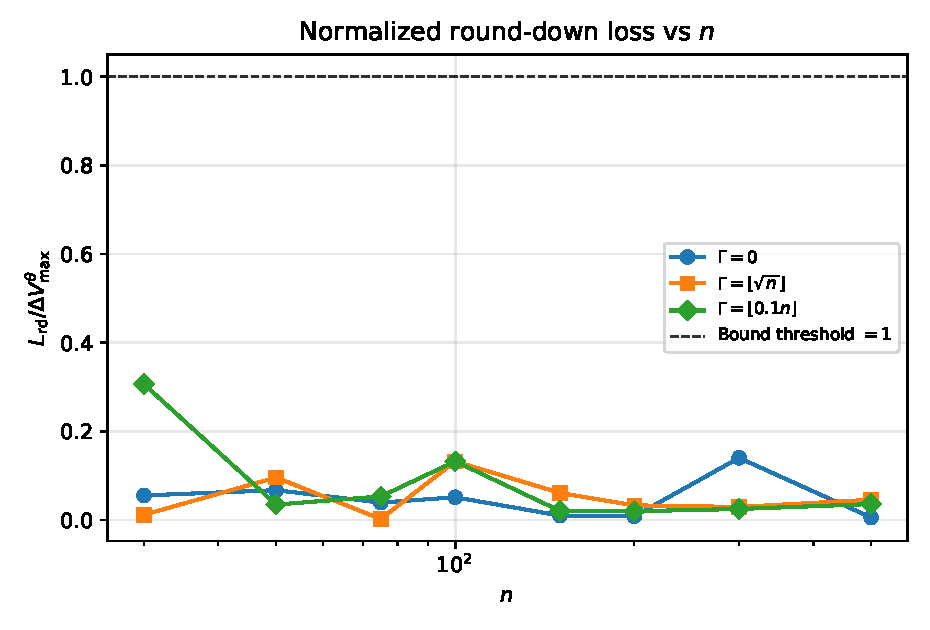
\includegraphics[width=\linewidth]{exp1/gap_loss_vs_n.pdf}\\
{\small (a) Normalized rounding loss $L_{\mathrm{rd}}/\Delta V_{\max}^\theta$ vs.\ $n$}
\end{minipage}\hfill
\begin{minipage}{0.48\textwidth}\centering
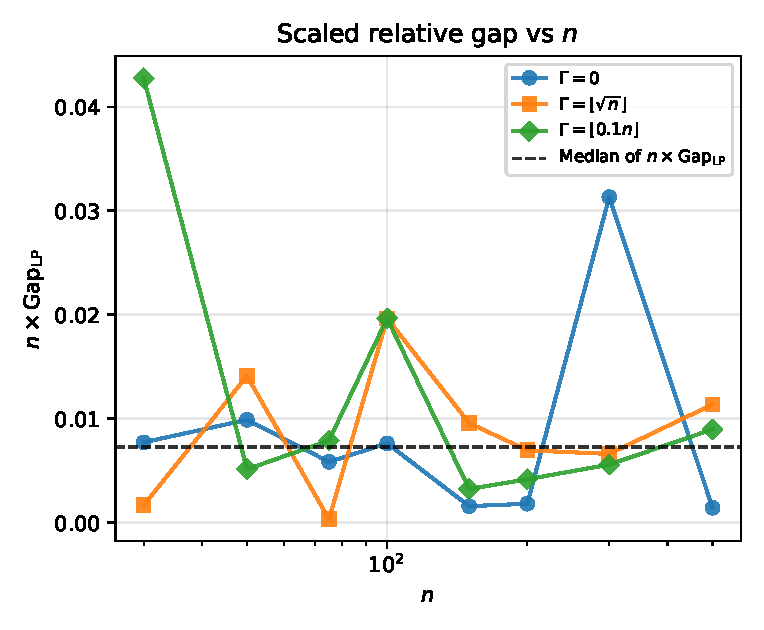
\includegraphics[width=\linewidth]{exp1/loss_vs_bound.pdf}\\
{\small (b) Scaled gap $n\times\mathrm{Gap}_{\mathrm{LP}}$ vs.\ $n$}
\end{minipage}
\caption{Integrality gap (\Cref{prop:igap_additive_theta_clean,cor:igap_relative_theta_clean}).
(a)~Ratio of round-down loss to additive bound vs.\ $n$ for three $\Gamma$-regimes; all points
lie well below the theoretical ceiling of~$1$ (dashed), consistent with
\Cref{prop:igap_additive_theta_clean}.
(b)~Scaled relative gap $n\times\mathrm{Gap}_{\mathrm{LP}}$ vs.\ $n$; the product fluctuates
around a stable median (dashed) with no upward trend, consistent with the \(O(1/n)\) decay of
\Cref{cor:igap_relative_theta_clean}.}
\label{fig:gap_decay}
\end{figure}
% ============================================================
% EXPERIMENT 2: SCALABILITY, HULL COMPRESSION, THETA ENUMERATION
% ============================================================
% ============================================================
% EXPERIMENT 2: SCALABILITY, HULL COMPRESSION, THETA ENUMERATION
% ============================================================
\subsection{Scalability, hull compression, and
\texorpdfstring{$\theta$}{theta}-enumeration efficiency}%
\label{subsec:numerics_scalability}

We assess the practical scalability of Algorithm~\ref{alg:robust_hull_greedy}, the compression
achieved by upper-hull filtering (\Cref{thm:master_greedy}(i)--(ii)), and the efficiency of the
$\theta$-enumeration (\Cref{prop:theta_candidates_discrete_clean}).

\paragraph{Runtime scaling.}
Fix $\alpha=0.10$, $\Gamma=\lfloor\sqrt n\rfloor$, and consider
\[
m\in\{10,50\},\qquad
n\in\{30,\,50,\,75,\,100,\,150,\,200,\,300,\,500\}.
\]
We record total wall-clock time and a per-phase breakdown (preprocessing, $\theta$-loop
overhead, hull computation, greedy filling, rounding, and certification).

\Cref{fig:scalability}a shows total runtime on log-log axes with separate curves per~$m$.
Both curves closely track the slope-$2$ reference line, indicating empirical scaling of
approximately $O(n^2 m)$---consistent with $|\mathcal B|=O(nm)$ candidates each requiring
$O(n)$ work for hull construction and greedy filling.
The $m=50$ curve sits roughly one order of magnitude above the $m=10$ curve at every~$n$,
reflecting the linear dependence on menu size.
At $n=500$ and $m=50$, the total runtime is approximately \SI{400}{\second}; for $m=10$ the
same portfolio size completes in roughly \SI{30}{\second}.

\Cref{fig:scalability}c presents the runtime breakdown at $m=50$ as a stacked bar chart.
Hull construction (red) is overwhelmingly the dominant phase, accounting for the vast majority
of wall-clock time at every~$n$. All other phases---preprocessing, $\theta$-loop overhead,
greedy LP filling, rounding, and certification---are negligible by comparison. This indicates
that hull construction is the computational bottleneck and that the sweep-style optimizations
described in \Cref{sec:algorithm} (restricting $\mathcal B$ to undominated breakpoints and
caching hulls for unchanged items) target the dominant phase.

\paragraph{Hull compression.}
Since hull structure is a per-item property that is essentially independent of portfolio
size~$n$, we evaluate hull compression on the $n=500$ master instance at $\theta=0$ for
$m\in\{10,20,50,100\}$; this requires only a single hull construction per item (no
$\theta$-enumeration) and is computationally negligible.

\Cref{fig:scalability}b shows the distribution of per-item hull sizes grouped by raw menu
size~$m$, with median values annotated. The median hull sizes are $7$, $13$, $33$, and $67$
for $m=10$, $20$, $50$, and $100$ respectively, corresponding to a compression ratio of
roughly two-thirds across all menu sizes. Dashed reference lines at the raw~$m$ values show
the gap between the full menu and the hull.
While the compression ratio is approximately constant in~$m$, the \emph{absolute} reduction
grows with menu size: at $m=100$ the hull discards a median of $33$ options per item,
directly reducing the size of the candidate set $\mathcal B$ and the per-$\theta$ hull
construction cost.

\paragraph{$\theta$-enumeration efficiency.}
For each instance we record $|\mathcal B|$ (after deduplication), the number of candidates
skipped due to $C^\theta<0$, and the number of distinct $\theta$-values at which the final
discrete objective $N(\bm x(\theta))$ strictly improves over the previous best.
In all configurations, a large fraction of candidates is skipped early ($C^\theta<0$), and
among the evaluated candidates only a small subset improves the incumbent objective. The skip
rate increases with portfolio size, consistent with the prediction of
\Cref{prop:theta_candidates_discrete_clean}. Combined with the hull compression above, these
two mechanisms---candidate reduction and early termination---help explain why the observed runtime
appears close to quadratic in $n$ for a fixed menu size $m$ on the tested instances, rather than reflecting the most pessimistic worst-case bound.

\paragraph{Box-case cross-check ($\Gamma=n$).}
As an additional structural validation, we verify that for $\Gamma=n$ (box uncertainty) the
general $\theta$-enumeration algorithm produces the same solution as directly solving the
separable formulation~\eqref{eq:box_problem}. On all tested prefix sizes the objectives match
to machine precision, validating both the theory of \Cref{sec:structure} and the
implementation.

\begin{figure}[H]
\centering
\begin{minipage}{0.32\textwidth}\centering
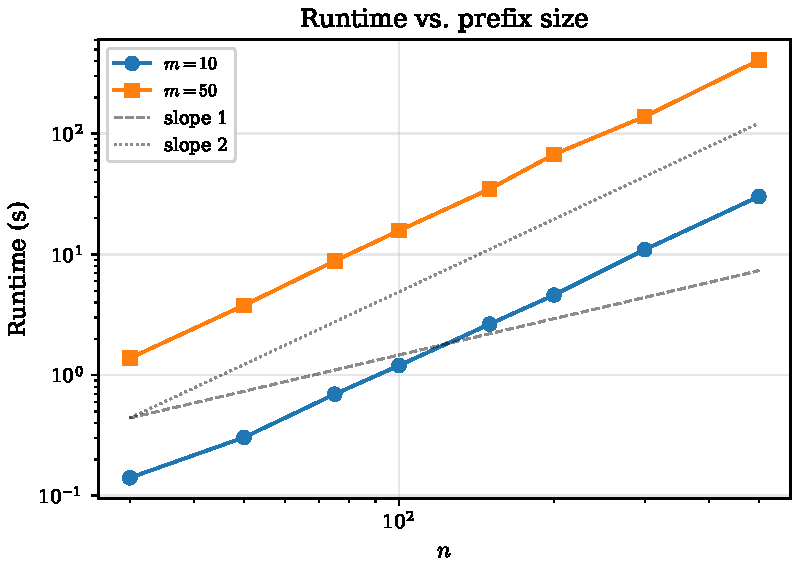
\includegraphics[width=\linewidth]{exp2/runtime_vs_n.pdf}\\
{\small (a) Runtime vs.\ $n$ (log-log)}
\end{minipage}\hfill
\begin{minipage}{0.32\textwidth}\centering
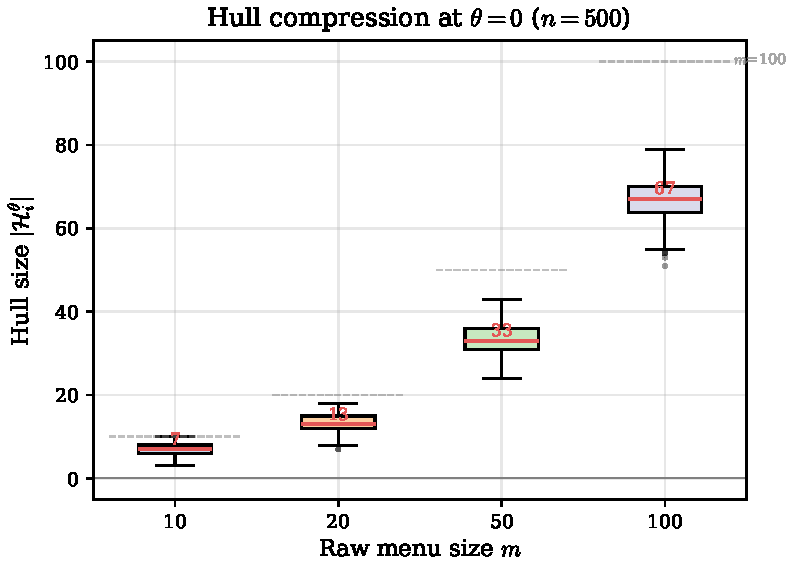
\includegraphics[width=\linewidth]{exp2/hull_sizes.pdf}\\
{\small (b) Hull size by $m$ ($n=500$)}
\end{minipage}\hfill
\begin{minipage}{0.32\textwidth}\centering
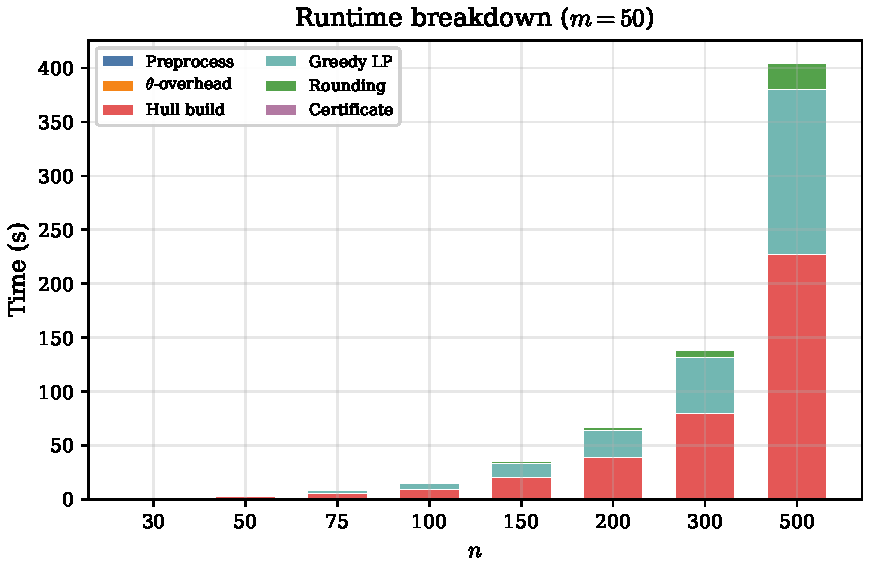
\includegraphics[width=\linewidth]{exp2/runtime_breakdown.pdf}\\
{\small (c) Runtime breakdown ($m=50$)}
\end{minipage}
\caption{Scalability and hull compression.
(a)~Wall-clock runtime of \Cref{alg:robust_hull_greedy} vs.\ $n$ for $m\in\{10,50\}$;
reference lines at slopes~$1$ and~$2$ are overlaid. Both curves track close to slope~$2$.
(b)~Box plot of per-item hull size $|\mathcal H_i^\theta|$ at $\theta=0$, grouped by raw menu
size~$m$, on the $n=500$ master instance; annotated values are medians. Dashed lines mark the
raw menu size for reference; the hull retains roughly two-thirds of the menu across all~$m$.
(c)~Stacked bar chart of runtime by algorithm phase ($m=50$); hull construction dominates at
every~$n$.}
\label{fig:scalability}
\end{figure}
% ============================================================
% EXPERIMENT 3: REVENUE--RISK FRONTIER
% ============================================================
% ============================================================
% EXPERIMENT 3: REVENUE--RISK FRONTIER
% ============================================================
\subsection{Revenue--risk frontier}\label{subsec:numerics_robustness}

We quantify the practical value of $\Gamma$-budget protection (\Cref{thm:robust}) and
investigate the tightness of the guarantee.

\paragraph{Frontier construction.}
Fix $n=200$ (the $200$-item prefix of the master portfolio), $m=50$,
$\alpha\in\{0.10,0.20\}$, and vary $\Gamma$ over
\[
\{0,\,1,\,3,\,5,\,10,\,\lfloor\sqrt{n}\rfloor,\,20,\,30,\,50,\,100,\,n\}.
\]
For each solution $\bm x$ we run $S=10\,000$ Monte Carlo stress scenarios under two
complementary perturbation protocols.

The first is an \textbf{adversarial (worst-case-direction)} stress test: by \Cref{thm:robust},
the margin constraint can only be violated when deviations oppose the sign of $t_i(x_i)$.
We sample $K\subset\{1,\dots,n\}$ with $|K|=\Gamma_{\mathrm{attack}}$ uniformly at random,
draw $\xi_i\sim\mathrm{Uniform}(-1,0)$ for $i\in K$, and set
$\xi_i':=\xi_i\cdot\operatorname{sgn}(t_i(x_i))$ so that each deviation opposes the margin
contribution; for $i\notin K$, $\xi_i':=0$.
The attack level for the frontier plots is
$\Gamma_{\mathrm{attack}}=\max(\Gamma,\,\lfloor1.5\Gamma\rfloor)$, which lies strictly
above the protection budget for $\Gamma>0$ and thus falls outside the certified uncertainty
set~$\mathcal U^\Gamma$.

The second is an \textbf{i.i.d.\ (stochastic)} stress test that models undirected demand
noise: for every item~$i$, independently draw $\xi_i\sim\mathrm{Uniform}(-1,1)$.
In both cases, realized demand is
$\tilde g_i(x_i)=\max\big(0,\;\hat g_i(x_i)+\xi_i'\,\delta_i(x_i)\big)$ and the realized
margin is $S_{\mathrm{realized}}=\sum_i\omega_i(x_i-\Delta a_i)\tilde g_i$.
We report violation probability
$\hat P:=S^{-1}\sum_{s=1}^S\ind[S_{\mathrm{realized}}^{(s)}<0]$ and the $5\%$-quantile of
$S_{\mathrm{realized}}$.

\paragraph{Sanity check: zero observed violations at matching attack level.}
By construction, \Cref{thm:robust} guarantees $S(\bm x)\ge 0$ for all realizations in
$\mathcal U^\Gamma$. Adversarial scenarios with $\Gamma_{\mathrm{attack}}=\Gamma$ lie within
$\mathcal U^\Gamma$ and should produce zero observed violations. We observe this on all $22$
configurations, providing a correctness check of both the certificate and the simulation.

\paragraph{Tightness of protection.}
To assess how tight the guarantee is, we additionally stress-test each
$\Gamma$-protected solution at attack levels
$\Gamma_{\mathrm{attack}}\in\{\Gamma,\;\Gamma+\lfloor0.1n\rfloor,\;2\Gamma,\;n\}$.
This shows that violations reappear once the attack exceeds the protection budget, directly
illustrating the ``price of robustness'' interpretation of \citet{BertsimasSim2004}.

\paragraph{Results.}
\Cref{fig:risk_frontier}a displays the revenue--risk frontier for $n=200$ as two vertically
aligned panels sharing a common $\Gamma/n$ axis.
The top panel shows normalized revenue: the cost of robustness is remarkably small, with
even full box protection ($\Gamma=n$) sacrificing less than $1\%$ of nominal revenue in the synthetic frontier experiment for
both $\alpha=0.10$ and $\alpha=0.20$. The revenue curve is smooth and concave,
indicating diminishing marginal cost of additional protection.
The bottom panel shows violation probability under both adversarial (solid) and i.i.d.\
(dashed) shocks at attack level $\Gamma_{\mathrm{attack}}=\max(\Gamma,\lfloor1.5\Gamma\rfloor)$.
The nominal solution ($\Gamma=0$) is highly vulnerable: adversarial violations reach
approximately $50\%$ and even undirected i.i.d.\ shocks produce violations roughly $30\%$ of
the time. Violations drop sharply to zero by $\Gamma/n\approx 0.05$ (i.e.\
$\Gamma\approx 10$), indicating that a modest protection budget covering $5\%$ of the
portfolio is sufficient to eliminate all observed violations under both perturbation protocols.

\Cref{fig:risk_frontier}b shows that the $5\%$-quantile of realized margin increases
monotonically with~$\Gamma$, with a concave profile: the steepest gains occur at small
$\Gamma/n$, after which the curve flattens as additional protection yields diminishing
tail-risk improvement. The $\alpha=0.20$ curve lies above $\alpha=0.10$ at every $\Gamma$
because larger uncertainty amplitude induces the robust algorithm to build a larger margin
buffer, resulting in a higher tail quantile under the adversarial stress test.

\Cref{fig:risk_frontier}c presents the tightness heatmap for $\alpha=0.10$: rows index the
protection level~$\Gamma$, columns index $\Gamma_{\mathrm{attack}}$, and color encodes
violation probability on a logarithmic scale.
Below and on the diagonal (dashed line at $\Gamma_{\mathrm{attack}}=\Gamma$) the heatmap is
white, indicating zero observed violations in line with \Cref{thm:robust}.
Above the diagonal, violation probability increases smoothly with the gap between attack and
protection levels, exhibiting the staircase structure predicted by the $\Gamma$-budget model:
each additional unit of protection shifts the white region one step further from the diagonal.

\begin{figure}[H]
\centering
\begin{minipage}{0.32\textwidth}\centering
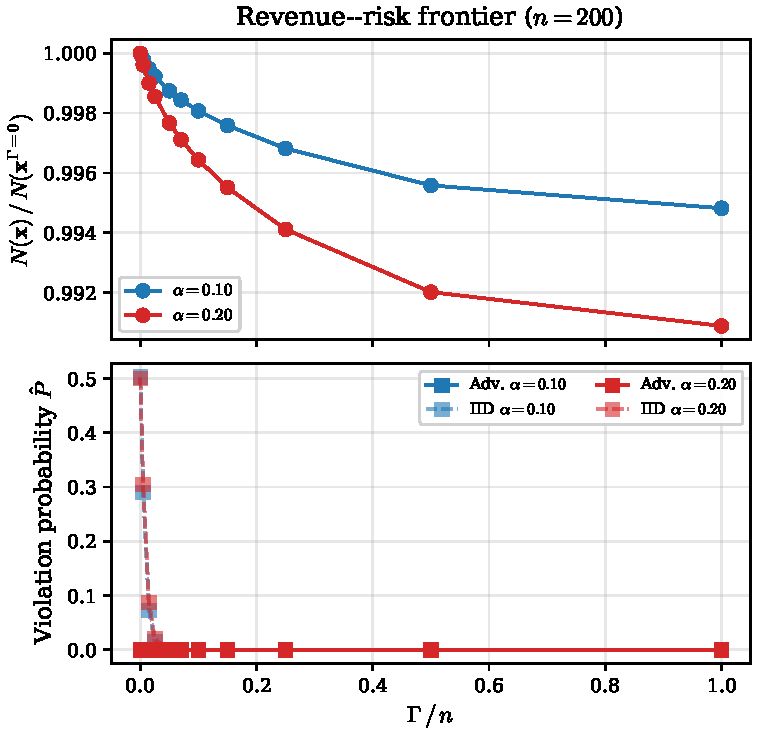
\includegraphics[width=\linewidth]{exp3/risk_frontier.pdf}\\
{\small (a) Revenue--violation frontier}
\end{minipage}\hfill
\begin{minipage}{0.32\textwidth}\centering
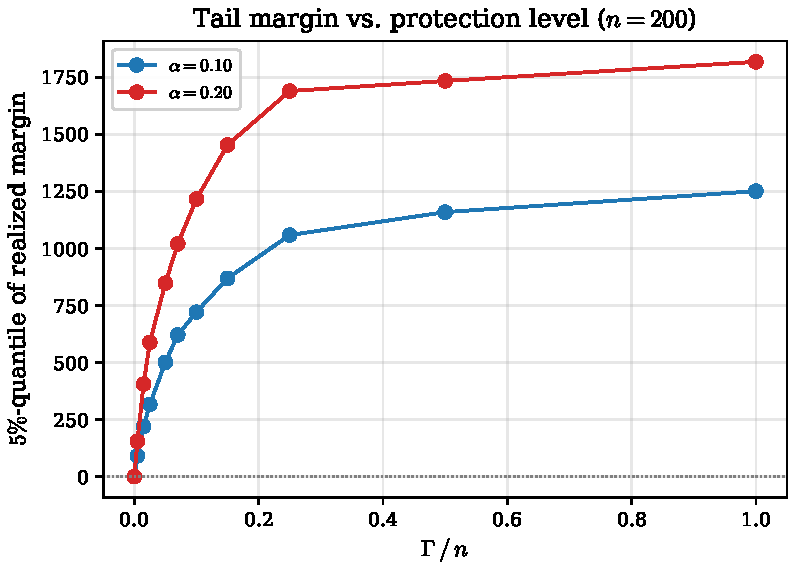
\includegraphics[width=\linewidth]{exp3/tail_margin.pdf}\\
{\small (b) $5\%$-quantile of margin}
\end{minipage}\hfill
\begin{minipage}{0.32\textwidth}\centering
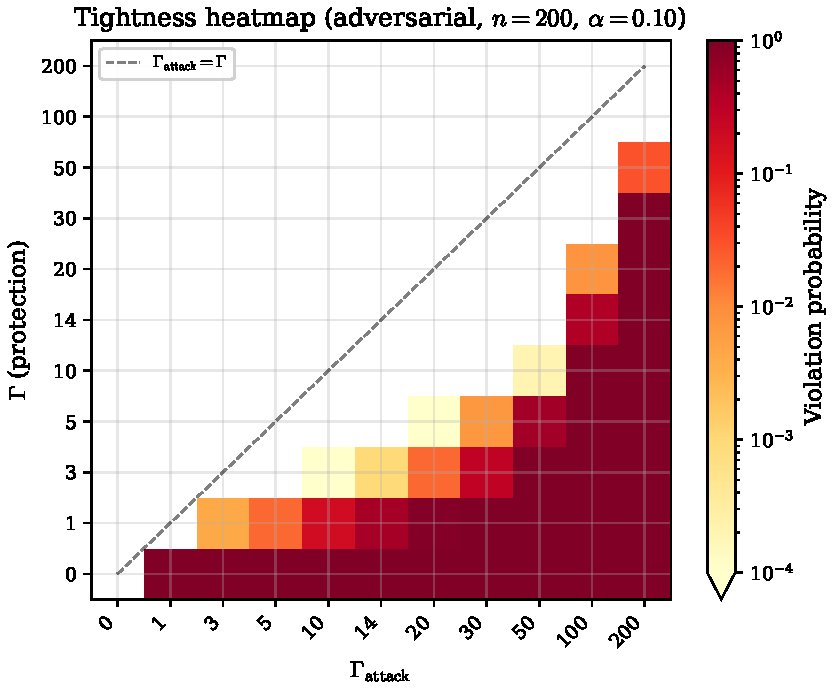
\includegraphics[width=\linewidth]{exp3/tightness_heatmap.pdf}\\
{\small (c) Tightness: protection vs.\ attack}
\end{minipage}
\caption{Revenue--risk frontier (\Cref{thm:robust}, $n=200$).
(a)~Top: normalized revenue $N(\bm x)/N(\bm x^{\Gamma=0})$; bottom: violation probability
$\hat P$ under adversarial shocks (solid) and i.i.d.\ shocks (dashed), for
$\alpha\in\{0.10,0.20\}$. Revenue cost is below $1\%$ even at $\Gamma=n$; violations vanish
by $\Gamma/n\approx 0.05$.
(b)~$5\%$-quantile of realized margin vs.\ $\Gamma/n$; higher $\alpha$ produces a larger
margin buffer and higher tail quantile.
(c)~Heatmap of violation probability (adversarial, $\alpha=0.10$, log scale): below the
diagonal $\Gamma_{\mathrm{attack}}=\Gamma$ (dashed) all cells are white (zero violations,
\Cref{thm:robust}); above the diagonal violations increase smoothly.}
\label{fig:risk_frontier}
\end{figure}
% ============================================================
% AGGREGATE TABLE
% ============================================================
% ============================================================
% EXPERIMENT 4: AGGREGATE SUMMARY TABLE
% ============================================================
\subsection{Aggregate summary}\label{subsec:numerics_table}

\Cref{tab:numerics_summary} consolidates representative configurations across scales and
uncertainty levels, using $\Gamma=\lfloor\sqrt{n}\rfloor$ throughout.
All reported solutions satisfy the robust constraint as certified by~\eqref{eq:certify_alg};
adversarial and i.i.d.\ stress tests at $S=10\,000$ scenarios show zero or negligible
violation rates.

The $L_{\mathrm{rd}}$ and $\Delta V_{\max}^\theta$ columns are consistent with the additive bound of
\Cref{prop:igap_additive_theta_clean} on every configuration: the rounding loss stays well
below the single-item bound, with ratios
$L_{\mathrm{rd}}/\Delta V_{\max}^\theta$ ranging from $0.01$ to $0.37$.
The relative gap $\mathrm{Gap}_{\mathrm{LP}}$ is of order $10^{-5}$--$10^{-4}$ throughout,
consistent with the \(O(1/n)\) decay established in \Cref{subsec:numerics_gap}.
Revenue sacrifice is minimal: the revenue ratio
$N(\bm x)/N(\bm x^{\Gamma=0})$ exceeds $0.997$ in all cases, indicating that
$\Gamma$-budget protection costs less than $0.3\%$ of nominal revenue in the representative configurations of \Cref{tab:numerics_summary}.
Runtime scales quadratically in~$n$ (roughly $4\,\text{s}\to 16\,\text{s}\to 65\,\text{s}
\to 410\,\text{s}$ for $n=50\to 500$), consistent with the scaling analysis of
\Cref{subsec:numerics_scalability}.

\begin{table}[H]
\centering
\caption{Representative performance across scales (nested prefixes from a single $n=500$
portfolio, $m=50$, $\Gamma=\lfloor\sqrt{n}\rfloor$).
$L_{\mathrm{rd}}$: absolute round-down loss;
$\Delta V_{\max}^\theta$: theoretical additive bound
(\Cref{prop:igap_additive_theta_clean});
$\mathrm{Gap}_{\mathrm{LP}}$: $L_{\mathrm{rd}}/\mathrm{OPT}_{\mathrm{LP}}$;
Rev.\ ratio: $N(\bm x)/N(\bm x^{\Gamma=0})$;
Viol.\ (adv.): $\hat P$ under adversarial shocks at
$\Gamma_{\mathrm{attack}}=\lfloor1.5\Gamma\rfloor$;
Viol.\ (iid): $\hat P$ under i.i.d.\ $\mathrm{Uniform}(-1,1)$ shocks
($S=10\,000$ scenarios).}
\label{tab:numerics_summary}
\small
\begin{tabular}{r r r r r r r r r r}
\toprule
$n$ & $\alpha$ & $\Gamma$ &
Time (s) &
$L_{\mathrm{rd}}$ &
$\Delta V_{\max}^\theta$ &
$\mathrm{Gap}_{\mathrm{LP}}$ &
Rev.\ ratio &
Viol.\ (adv.) &
Viol.\ (iid) \\
\midrule
% --- n = 50 ---
$50$ & $0.10$ & $7$
 & $3.79$ & $52.5$ & $547$ & $2.8\!\times\!10^{-4}$ & $0.998$ & $0$ & $5\!\times\!10^{-4}$ \\
$50$ & $0.20$ & $7$
 & $3.89$ & $14.4$ & $547$ & $7.8\!\times\!10^{-5}$ & $0.997$ & $0$ & $2\!\times\!10^{-3}$ \\
\midrule
% --- n = 100 ---
$100$ & $0.10$ & $10$
 & $16.2$ & $72.4$ & $547$ & $2.0\!\times\!10^{-4}$ & $0.999$ & $0$ & $0$ \\
$100$ & $0.20$ & $10$
 & $15.8$ & $5.08$ & $547$ & $1.4\!\times\!10^{-5}$ & $0.998$ & $0$ & $5\!\times\!10^{-4}$ \\
\midrule
% --- n = 200 ---
$200$ & $0.10$ & $14$
 & $62.0$ & $25.9$ & $782$ & $3.5\!\times\!10^{-5}$ & $0.999$ & $0$ & $0$ \\
$200$ & $0.20$ & $14$
 & $68.6$ & $287$ & $782$ & $3.9\!\times\!10^{-4}$ & $0.998$ & $0$ & $0$ \\
\midrule
% --- n = 500 ---
$500$ & $0.10$ & $22$
 & $412$ & $44.4$ & $968$ & $2.3\!\times\!10^{-5}$ & $0.999$ & $0$ & $0$ \\
$500$ & $0.20$ & $22$
 & $401$ & $92.9$ & $968$ & $4.8\!\times\!10^{-5}$ & $0.998$ & $0$ & $0$ \\
\bottomrule
\end{tabular}
\par\vspace{2pt}
\footnotesize\emph{Note:} The identical value of 547 for $\Delta V_{\max}^\theta$ at $n=50$ and $n=100$ is a direct result of the deterministic nested prefix instance design.
\end{table}

% ============================================================
% LIMITATIONS (closing paragraph of §Numerical Results)
% ============================================================
\paragraph{Limitations.}
Several design choices bound the scope of the experiments above.
First, all instances derive from a single synthetic demand model (piecewise-linear with
proportional uncertainty) and a single master portfolio; while the generator produces
realistic heterogeneity across items, validation on observed pricing data---retail scanner
panels, insurance tariffs, or online marketplace catalogs---would test the hull-filtering
and rounding machinery under distributional features (e.g.\ multi-modal demand, correlated
perturbations) that the current generator does not produce.
Second, the nested-prefix design eliminates cross-instance sampling variation and cleanly
isolates the effect of portfolio size, but it means every $n$-configuration shares the same
first~$n$ items; independent random instances with multiple replicates would provide
complementary evidence on average-case behavior.
Third, portfolio sizes are capped at $n=500$ by the $O(n^2 m)$ cost of na\"ive
$\theta$-enumeration (\Cref{subsec:numerics_scalability}); the sweep-style optimizations
of \Cref{sec:algorithm}---restricting candidates to undominated breakpoints and caching
hulls incrementally---may extend the practical frontier to $n\ge 10^4$ but
are not yet implemented.
% ============================================================
% SECTION: STYLIZED APPLICATION (GROCERY PRICING)
% ============================================================
% ============================================================
% SECTION: STYLIZED APPLICATION — RETAIL CATEGORY PRICING
% ============================================================
% ============================================================
% CASE STUDY: CATEGORY PRICING IN RETAIL
% ============================================================
\section{Stylized Application: Category Pricing in Retail}\label{sec:case_study}

To illustrate the managerial value of the $\Gamma$-budget robust framework beyond the
controlled synthetic setting of \Cref{sec:numerics}, we analyze a stylized retail grocery
pricing problem with economically calibrated parameters, non-linear demand, and
heterogeneous uncertainty.

Consider a category manager responsible for setting regular (non-promotional) shelf prices for
a portfolio of $n=300$ Stock Keeping Units (SKUs) spanning a mid-size grocery category such as
dairy, breakfast, or household cleaning. The manager faces a quarterly gross-margin target
$\Delta$ dictated by corporate planning, but demand is susceptible to disruptions: unannounced
competitor promotions, supply-chain cost shocks, and shifts in consumer preference between
national brands and private-label substitutes.

% ============================================================
\subsection{Economic model and portfolio construction}
\label{subsec:case_model}

\paragraph{Portfolio structure.}
To capture the heterogeneity typical of a grocery category, we partition the $300$ SKUs into
four segments that reflect standard retail assortment tiers:

\begin{enumerate}
\item \textbf{Staples} ($120$ SKUs): high-volume, low-margin essentials (e.g.\ whole milk,
  white bread, eggs) with low price sensitivity. Reference prices
  $a_i\sim\exp\bigl(\mathcal N(\mu{=}\log 3.0,\,\tau^2{=}0.15)\bigr)$, median $\approx\$3.00$.
\item \textbf{Mainstream brands} ($100$ SKUs): mid-range national-brand products (e.g.\
  branded yogurt, cereal, pasta sauce) with moderate elasticity. Reference prices
  $a_i\sim\exp\bigl(\mathcal N(\mu{=}\log 5.5,\,\tau^2{=}0.20)\bigr)$, median $\approx\$5.50$.
\item \textbf{Premium \& specialty} ($50$ SKUs): higher-priced items with larger absolute
  margins but smaller volume (e.g.\ organic produce, artisanal cheese, specialty beverages).
  Reference prices $a_i\sim\exp\bigl(\mathcal N(\mu{=}\log 9.0,\,\tau^2{=}0.25)\bigr)$, median $\approx\$9.00$.
\item \textbf{Private label} ($30$ SKUs): store-brand alternatives to mainstream products,
  positioned on price and highly exposed to competitive price gaps. Reference prices
  $a_i\sim\exp\bigl(\mathcal N(\mu{=}\log 3.5,\,\tau^2{=}0.10)\bigr)$, median $\approx\$3.50$.
\end{enumerate}

\paragraph{Demand model.}
Consumer response in retail grocery is well described by a constant-elasticity (iso-elastic)
demand function with a segment-dependent volume anchor.
For each SKU~$i$ in segment~$k$, the nominal demand reaction function is
\begin{equation}\label{eq:case_demand}
  \hat g_i(x_i)
  \;=\; d_i\!\left(\frac{x_i}{a_i}\right)^{\!-\eta_i},
\end{equation}
where $d_i$ is the baseline weekly unit volume at reference price $a_i$ and $\eta_i>1$ is the
price elasticity. We draw the segment-specific parameters as follows:
\[
\renewcommand{\arraystretch}{1.15}
\begin{array}{lccl}
\toprule
\textbf{Segment} & \eta_i & d_i & \textbf{Rationale}\\
\midrule
\text{Staples}
  & \mathrm{Uniform}(1.2,\,2.0)
  & \exp\bigl(\mathcal N(\mu{=}\log 150,\,\tau^2{=}0.30)\bigr)
  & \text{inelastic; high turns}\\
\text{Mainstream}
  & \mathrm{Uniform}(2.0,\,3.5)
  & \exp\bigl(\mathcal N(\mu{=}\log 60,\,\tau^2{=}0.35)\bigr)
  & \text{moderate sensitivity}\\
\text{Premium}
  & \mathrm{Uniform}(1.5,\,2.5)
  & \exp\bigl(\mathcal N(\mu{=}\log 20,\,\tau^2{=}0.40)\bigr)
  & \text{niche; low volume}\\
\text{Private label}
  & \mathrm{Uniform}(3.0,\,5.0)
  & \exp\bigl(\mathcal N(\mu{=}\log 80,\,\tau^2{=}0.25)\bigr)
  & \text{price-driven switching}\\
\bottomrule
\end{array}
\]
The iso-elastic form~\eqref{eq:case_demand} generates a revenue curve
$r_i(x_i) = x_i\,\hat g_i(x_i) = d_i\,a_i^{\eta_i}\,x_i^{1-\eta_i}$ that is concave in $x_i$
when $\eta_i>1$, but the per-item margin contribution
$s_i(x_i) = \omega_i(x_i - \Delta a_i)\hat g_i(x_i)$, when evaluated over a discrete menu,
need not trace a concave envelope in the cost--value plane, making the upper-hull filtering
of \Cref{subsec:hull_lp} essential.

\paragraph{Exposures and margin target.}
We set $\omega_i = d_i / \bar d$ where $\bar d$ is the portfolio mean of $d_i$, so that the
margin constraint weights each SKU by its volume share---reflecting the standard retail
practice of measuring category margin on a revenue-weighted basis.
The margin target~$\Delta$ is calibrated to represent a gross-margin hurdle of approximately
$30\%$:
\[
\Delta \;=\; (1 - 0.02)\,
\frac{\sum_{i=1}^n \omega_i\,\tilde x_i\,\hat g_i(\tilde x_i)}%
     {\sum_{i=1}^n \omega_i\,a_i\,\hat g_i(\tilde x_i)},
\]
with $\tilde x_i$ the menu point closest to $a_i$. The $2\%$ relative slack
(cf.\ \Cref{subsec:numerics_protocol}) ensures feasibility across the full $\Gamma$-grid;
we verify this on all tested configurations.

\paragraph{Discrete price menus.}
For each SKU~$i$ we construct $m=20$ candidate price points within the admissible band
$[(1-\sigma_i)a_i,\;(1+\sigma_i)a_i]$ with $\sigma_i = 0.10$. Rather than spacing prices
uniformly, we adopt a retailer-realistic grid that respects psychological price endings:
each candidate is rounded to the nearest cent ending in $\$.X9$ (i.e.\ \$2.49, \$3.99,
\$5.19, etc.) and then deduplicated. This produces menus with slightly irregular spacing and
occasionally fewer than $m$ distinct options for low-priced staples, since a $\pm10\%$ band
around $\$3.00$ offers less price granularity than the same band around $\$9.00$.

\paragraph{Demand uncertainty.}
We model heterogeneous uncertainty that reflects the distinct risk profiles of each segment.
The deviation bound is $\delta_i(x_i) = \alpha_i\,\hat g_i(x_i)$, with segment-specific
uncertainty levels:
\[
\renewcommand{\arraystretch}{1.15}
\begin{array}{lcl}
\toprule
\textbf{Segment} & \alpha_i & \textbf{Rationale}\\
\midrule
\text{Staples} & 0.08
  & \text{stable demand; low substitution risk}\\
\text{Mainstream} & 0.15
  & \text{exposed to promotional warfare}\\
\text{Premium} & 0.12
  & \text{niche loyalty; moderate shock exposure}\\
\text{Private label} & 0.25
  & \text{high cross-price sensitivity; competitor-driven}\\
\bottomrule
\end{array}
\]
This heterogeneity is important: a uniform $\alpha$ would understate risk for
price-sensitive private-label SKUs and overstate it for inelastic staples. Under the
$\Gamma$-budget model, the adversary selects the \emph{most damaging} $\Gamma$ items to
perturb, so high-$\alpha_i$ SKUs with large margin contributions become the natural attack
surface. The theoretical guarantees of \Cref{thm:robust} and
\Cref{prop:igap_additive_theta_clean} hold for any parameter realization; only the magnitude
of the revenue--risk tradeoff depends on the specific instance.

% ============================================================
\subsection{Experimental design}
\label{subsec:case_experiment}

We generate the $n=300$ portfolio from a single seed (master seed~$42$) and solve the robust
MCKP at
\[
\Gamma \in \{0,\,1,\,5,\,10,\,15,\,\lfloor\sqrt{n}\rfloor{=}17,\,30,\,50,\,75,\,100,\,n\}
\]
using \Cref{alg:robust_hull_greedy}.
For each $\Gamma$-level we record the nominal objective, wall-clock time, rounding loss
$L_{\mathrm{rd}}$, and the number of SKUs whose optimal price shifts relative to the
$\Gamma=0$ solution.
Each solution is stress-tested with $S=10\,000$ Monte Carlo scenarios under both the
adversarial and i.i.d.\ perturbation protocols defined in \Cref{subsec:numerics_robustness},
with $\Gamma_{\mathrm{attack}} \in \{\Gamma,\,\lfloor1.5\Gamma\rfloor,\,2\Gamma,\,n\}$.



% ============================================================
\subsection{Managerial insights}
\label{subsec:case_insights}

\paragraph{Concentration risk under nominal pricing.}
When optimizing nominally ($\Gamma=0$), the MCKP fulfills the category margin target by
extracting surplus from a concentrated subset of inelastic items. In the generated instance,
of the $300$ SKUs only $68$ have non-trivial margin contributions (above the $25$th percentile
of positive contributions)---predominantly staples and a handful of premium items that are
upgraded above their reference price. This pricing architecture is mathematically optimal under
perfect demand foresight but creates a fragile margin structure: the top-$\Gamma$ contributors
account for a disproportionate share of the margin surplus, so even a modest number of
simultaneous demand shocks can breach the category target.

Under i.i.d.\ stochastic shocks ($\xi_i\sim\mathrm{Uniform}(-1,1)$ independently for all
$300$ items), the nominal solution already exhibits a violation rate of approximately
$50\%$ (a coincidence distinct from the $50\%$ adversarial rate observed in \Cref{subsec:numerics_robustness}, driven here by heterogeneous uncertainty profiles)---the margin target is breached in half of all scenarios. Under worst-case-direction
adversarial shocks at $\Gamma_{\mathrm{attack}}=n$, the violation rate reaches $100\%$.
These numbers underscore that the nominal solution, while revenue-optimal, is operationally
unacceptable for a category manager facing any demand uncertainty.

\paragraph{Structural diversification under $\Gamma$-protection.}
Applying the robust algorithm with a modest budget ($\Gamma=17\approx\lfloor\sqrt{n}\rfloor$,
protecting against simultaneous shocks to roughly $6\%$ of the portfolio) produces a
qualitatively different pricing architecture (\Cref{fig:case_study}b). The robust solution:
\begin{itemize}
\item \emph{Spreads margin contributions} across a broader base: the number of SKUs with
  non-trivial margin contribution increases from $68$ to $76$ ($12\%$ increase) relative to
  the nominal solution;
\item \emph{Moderates prices on high-exposure items}: $39$ of $300$ SKUs shift price relative
  to the nominal solution, with private-label SKUs---which carry the largest per-unit
  uncertainty ($\alpha_i=0.25$)---seeing the largest downward adjustments, reducing their
  individual contribution to worst-case margin loss;
\item \emph{Preserves nearly all nominal revenue}: the revenue sacrifice is $0.28\%$ of the
  $\Gamma=0$ objective, well within the noise of typical weekly demand fluctuations.
\end{itemize}
This illustrates the core managerial tradeoff of the $\Gamma$-budget approach: by sacrificing
a fraction of a percent of expected revenue, the category manager structurally diversifies
margin risk away from a concentrated set of vulnerable SKUs.

\paragraph{Guidance on choosing $\Gamma$ in practice.}
The budget parameter $\Gamma$ controls the number of simultaneous worst-case demand deviations the solution must withstand. \citet{BertsimasSim2004} show that if individual deviations are independent and symmetrically distributed, the probability that more than $\Gamma$ items simultaneously reach their worst case is bounded above by a quantity that decays exponentially in $\Gamma^2/n$. For the $300$-SKU portfolio, $\Gamma=17\approx\lfloor\sqrt{n}\rfloor$ already provides a nontrivial level of probabilistic coverage under this bound. In practice, calibration should still be guided by historical demand data and scenario analysis, since the Bertsimas--Sim bound is conservative and the stress tests considered here are stylized. A category manager can calibrate $\Gamma$ empirically by examining historical demand data: if past records show that at most $K$ SKUs have simultaneously experienced demand drops exceeding one standard error of the demand estimate in any given week, then setting $\Gamma \geq K$ provides an empirically grounded protection level. The revenue--risk frontier in \Cref{fig:case_study}(a) supports this calibration by visualizing the marginal revenue cost of each additional unit of~$\Gamma$, allowing the manager to select the point on the frontier that best balances revenue performance against margin-breach risk tolerance.

\paragraph{Effectiveness of protection.}
\Cref{fig:case_study}a displays the revenue--risk frontier as two vertically aligned panels.
The top panel shows that the cost of robustness is remarkably small: even full box protection
($\Gamma=n=300$) sacrifices less than $0.7\%$ of nominal revenue in the stylized retail case study.
The bottom panel shows violation probability under adversarial and i.i.d.\ shocks.
Under i.i.d.\ shocks, the $51\%$ violation rate of the nominal solution drops below $0.2\%$
at $\Gamma=5$ (i.e.\ $\Gamma/n\approx 0.02$) and to zero for $\Gamma\ge 10$.
Under adversarial shocks at $\Gamma_{\mathrm{attack}}=\lfloor1.5\Gamma\rfloor$ (strictly
exceeding the protection budget for $\Gamma>0$), the observed violation rate is zero for all $\Gamma\ge 1$,
indicating that even minimal protection eliminates all observed adversarial violations at
moderate over-attack levels.

At the matching attack level ($\Gamma_{\mathrm{attack}}=\Gamma$), all $10\,000$ adversarial
scenarios produce zero observed violations for every tested~$\Gamma$, consistent with the certificate of
\Cref{thm:robust} and serving as an end-to-end correctness check.

\paragraph{Rounding-loss guarantee.}
The rounding loss satisfies $L_{\mathrm{rd}} < \Delta V_{\max}^\theta$ on every
configuration, with a ratio $L_{\mathrm{rd}}/\Delta V_{\max}^\theta = 0.023$ at
$\Gamma=\lfloor\sqrt{n}\rfloor$, consistent with the bound in
\Cref{prop:igap_additive_theta_clean} for this non-linear iso-elastic demand setting.

\paragraph{Operational practicality.}
Algorithm~\ref{alg:robust_hull_greedy} solves the $n=300$, $m=20$ instance in approximately
$18$ seconds for the tested $\Gamma$-values. While not instantaneous, this runtime is compatible with periodic repricing workflows such as weekly or batch updates when cost files or demand estimates are refreshed. Sweep-style optimizations of the type discussed in \Cref{sec:algorithm} may reduce runtime further, but these improvements are not yet implemented here.

\begin{figure}[H]
\centering
\begin{minipage}{0.48\textwidth}\centering
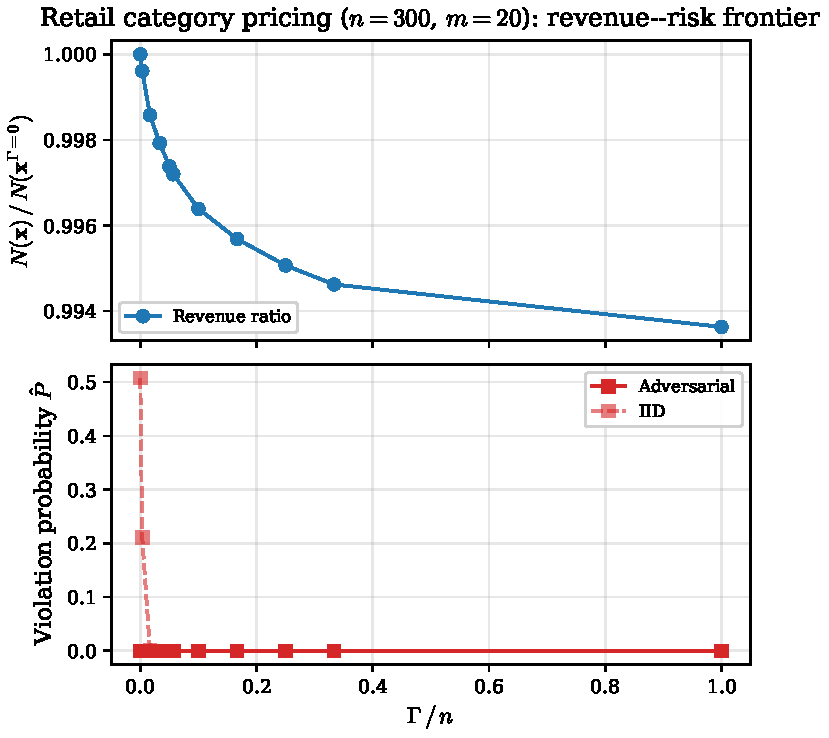
\includegraphics[width=\linewidth]{retail_pricing/case_frontier.pdf}\\
{\small (a) Revenue--violation frontier}
\end{minipage}\hfill
\begin{minipage}{0.48\textwidth}\centering
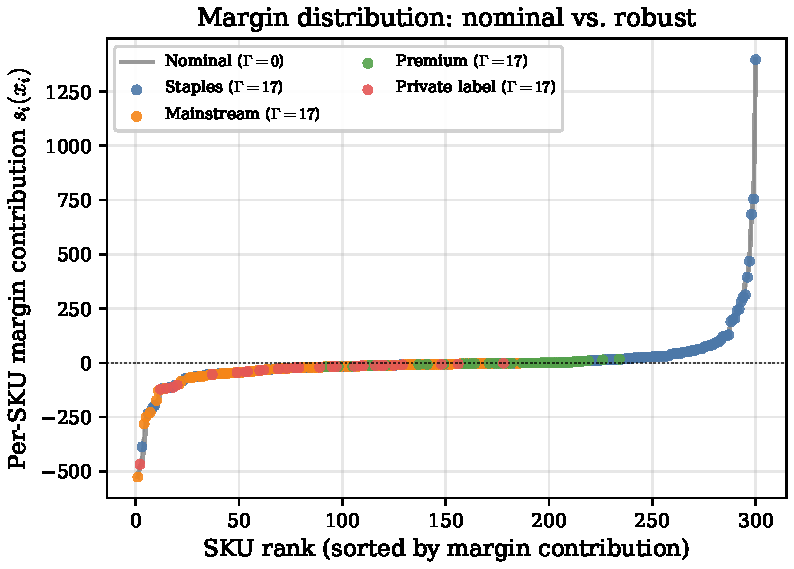
\includegraphics[width=\linewidth]{retail_pricing/case_margin_dist.pdf}\\
{\small (b) Per-SKU margin contribution}
\end{minipage}
\caption{Retail category pricing ($n=300$, $m=20$, heterogeneous $\alpha_i$).
(a)~Top: normalized category revenue $N(\bm x)/N(\bm x^{\Gamma=0})$; bottom: violation
probability $\hat P$ under adversarial shocks at
$\Gamma_{\mathrm{attack}}=\lfloor1.5\Gamma\rfloor$ (solid) and i.i.d.\ shocks (dashed).
Revenue cost is below $0.7\%$ even at $\Gamma=n$; i.i.d.\ violations vanish by
$\Gamma/n\approx0.03$.
(b)~Sorted per-SKU margin contribution $s_i(x_i)$ for the nominal solution ($\Gamma=0$,
gray) and the robust solution ($\Gamma=17\approx\lfloor\sqrt{n}\rfloor$, colored by segment).
The robust solution compresses the right tail and spreads positive contributions across a
broader SKU base.}
\label{fig:case_study}
\end{figure}
% ============================================================
% CONCLUSION
% ============================================================
\section{Conclusion}\label{sec:conclusion}

We have studied discrete pricing under demand uncertainty through the lens of robust
optimization, reducing the problem to a multiple-choice knapsack problem with a
$\Gamma$-budget uncertainty set in the capacity constraint.
Three main contributions emerge from this reduction.

First, we established that the LP relaxation of the fixed-$\theta$ subproblem admits an
additive integrality gap bounded by a single item's maximum hull-value jump
$\Delta V_{\max}^\theta$ (\Cref{prop:igap_additive_theta_clean}). Under the boundedness and linear-growth assumptions of \Cref{cor:igap_relative_theta_clean}, this yields a relative gap that decays as \(O(1/n)\).

Second, we showed that the $\Gamma$-budget robust constraint admits an exact reformulation
via $\theta$-enumeration over a finite set of breakpoints
(\Cref{thm:parametric,prop:theta_candidates_discrete_clean}), preserving the combinatorial structure that makes the
hull-greedy approach applicable. The resulting procedure avoids relying on a generic integer-programming solver in its main loop and exhibits close-to-$O(n^2 m)$ empirical scaling on the instances tested.

Third, numerical experiments on nested synthetic portfolios ($n$ up to $500$, $m$ up to
$100$) and a stylized retail application ($n=300$ SKUs, four segments, heterogeneous
uncertainty) are consistent with these theoretical properties on the tested instances.
Across these experiments, the observed integrality gap is negligible, $\Gamma$-budget
protection reduces or eliminates observed margin violations at a revenue cost below $1\%$ in the synthetic frontier experiment and in the stylized retail case study, and the algorithm solves the reported instances in seconds to minutes.

Several directions remain open.
Implementing the sweep-style optimizations of \Cref{sec:algorithm}---restricting
$\theta$-candidates to undominated breakpoints and caching hulls incrementally---may reduce runtime by one to two orders of magnitude, making portfolios with
$n\ge 10^4$ items tractable.
Extending the uncertainty model to capture cross-item demand correlations (e.g.\ through
factor-based or ellipsoidal sets) would broaden applicability to settings where
substitution effects dominate. A natural starting point is a factor model $\delta_i(x_i) = \bar\delta_i(x_i) + \beta_i \zeta$ where $\zeta$
is a common shock and $\beta_i$ are factor loadings; the resulting uncertainty set is an intersection of a $\Gamma$-budget set with an
ellipsoidal constraint, and the parametric decomposition of \Cref{thm:parametric} may admit an extension to this setting via a higher-dimensional dual representation.
Validation on observed transaction-level pricing data remains an important next step.


\section*{Data and Code Availability}
To facilitate reproducibility, the solver implementation and the code used to generate the reported numerical experiments are publicly available on GitHub:
\begin{center}
\url{https://github.com/eric939/robust_mckp}
\end{center}

\paragraph{Acknowledgments.} The author thanks Prof. Dr. Angela Kunoth (Department of Mathematics, University of Cologne) for her guidance and support. The problem was posed by Dr. Christian Mollet (Hannoversche Versicherung, Hannover, Germany), and the author also thanks him and his colleagues for several helpful discussions.

% ---------- References ----------
\newpage

\begin{thebibliography}{99}

\bibitem[Ben-Tal and Nemirovski(1999)]{BenTal1999}
Ben-Tal, A. and Nemirovski, A. (1999).
\newblock Robust solutions of uncertain linear programs.
\newblock \emph{Operations Research Letters}, 25(1), 1--13.
\newblock \url{https://doi.org/10.1016/S0167-6377(99)00016-4}.

\bibitem[Bertsimas and Sim(2004)]{BertsimasSim2004}
Bertsimas, D. and Sim, M. (2004).
\newblock The price of robustness.
\newblock \emph{Operations Research}, 52(1), 35--53.
\newblock \url{https://doi.org/10.1287/opre.1030.0065}.

\bibitem[Boukhari and Hifi(2023)]{Boukhari2023}
Boukhari, S. and Hifi, M. (2023).
\newblock An exact algorithm for the multiple-choice knapsack problem with setups.
\newblock \emph{Computers \& Industrial Engineering}, 188, 109818.
\newblock \url{https://doi.org/10.1016/j.cie.2023.109818}.

\bibitem[Boukhari and Hifi(2024)]{Boukhari2024}
Boukhari, S. and Hifi, M. (2024).
\newblock Combining local branching and descent method for solving the multiple-choice knapsack problem with setups.
\newblock \emph{International Transactions in Operational Research}, 31(1), 29--52.
\newblock \url{https://doi.org/10.1111/itor.13326}.

\bibitem[Caserta and Vo{\ss}(2019)]{Caserta2019}
Caserta, M. and Vo{\ss}, S. (2019).
\newblock The robust multiple-choice multidimensional knapsack problem.
\newblock \emph{Omega}, 86, 16--27.
\newblock \url{https://doi.org/10.1016/j.omega.2018.06.014}.

\bibitem[Dyer(1984)]{Dyer1984}
Dyer, M.~E. (1984).
\newblock An $O(n)$ algorithm for the multiple-choice knapsack linear program.
\newblock \emph{Mathematical Programming}, 29(1), 57--63.
\newblock \url{https://doi.org/10.1007/BF02592083}.

\bibitem[Goerigk et~al.(2021)]{Goerigk2021}
Goerigk, M., Lendl, S., and Wulf, L. (2021).
\newblock Robust combinatorial optimization with locally budgeted uncertainty.
\newblock \emph{Open Journal of Mathematical Optimization}, 2, Article~3.
\newblock \url{https://doi.org/10.5802/ojmo.5}.

\bibitem[Hamzeei et~al.(2022)]{Hamzeei2022}
Hamzeei, M., Lim, A., and Xu, J. (2022).
\newblock Robust price optimization of multiple products under interval uncertainties.
\newblock \emph{Journal of Revenue and Pricing Management}, 21(4), 442--454.
\newblock \url{https://doi.org/10.1057/s41272-021-00351-w}.

\bibitem[Ibaraki et~al.(1978)]{Ibaraki1978}
Ibaraki, T., Hasegawa, T., Teranaka, K., and Iwase, J. (1978).
\newblock The multiple-choice knapsack problem.
\newblock \emph{Journal of the Operations Research Society of Japan}, 21(1), 59--95.
\newblock \url{https://doi.org/10.15807/jorsj.21.59}.

\bibitem[Kellerer et~al.(2004)]{Kellerer2004}
Kellerer, H., Pferschy, U., and Pisinger, D. (2004).
\newblock \emph{Knapsack Problems}.
\newblock Springer.

\bibitem[Monaci et~al.(2013)]{Monaci2013}
Monaci, M., Pferschy, U., and Serafini, P. (2013).
\newblock Exact solution of the robust knapsack problem.
\newblock \emph{Computers \& Operations Research}, 40(11), 2625--2631.
\newblock \url{https://doi.org/10.1016/j.cor.2013.05.005}.

\bibitem[Nauss(1978)]{Nauss1978}
Nauss, R.~M. (1978).
\newblock The 0--1 knapsack problem with multiple choice constraints.
\newblock \emph{European Journal of Operational Research}, 2(2), 125--131.
\newblock \url{https://doi.org/10.1016/0377-2217(78)90108-X}.

\bibitem[Pisinger(1995)]{Pisinger1995}
Pisinger, D. (1995).
\newblock A minimal algorithm for the multiple-choice knapsack problem.
\newblock \emph{European Journal of Operational Research}, 83(2), 394--410.
\newblock \url{https://doi.org/10.1016/0377-2217(95)00015-I}.

\bibitem[Sinha and Zoltners(1979)]{Sinha1979}
Sinha, P. and Zoltners, A.~A. (1979).
\newblock The multiple-choice knapsack problem.
\newblock \emph{Operations Research}, 27(3), 503--515.
\newblock \url{https://doi.org/10.1287/opre.27.3.503}.

\end{thebibliography}

% ---------- Appendix ----------
\appendix
\section{Knapsack Problem}\label{app:background}

\paragraph{Classical 0--1 Knapsack.}
Given items $i=1,\dots,n$ with value $v_i\ge 0$ and cost $c_i\ge 0$, and a capacity $C$, the 0--1 knapsack problem is
\begin{align}
\max \quad & \sum_{i=1}^n v_i\,y_i \\
\text{s.t.}\quad & \sum_{i=1}^n c_i\,y_i \le C, \\
& y_i \in\{0,1\}\quad (i=1,\dots,n).
\end{align}

\paragraph{Multiple-Choice Knapsack (MCKP).}
This problem was first introduced by \citet{Nauss1978} as a generalization of the classical knapsack problem. Items are partitioned into $n$ groups; from each group exactly one option must be chosen.
Let group $i$ have discrete options (price levels) indexed by $j$, with value $v_{ij}$ and cost $c_{ij}$. With capacity $C$, the MCKP is
\begin{align}
    \max \quad & \sum_{i=1}^n \sum_j v_{ij}\,z_{ij} \label{eq:mckp_obj}\\
    \text{s.t.}\quad & \sum_{i=1}^n \sum_j c_{ij}\,z_{ij} \le C, \label{eq:mckp_cap}\\
    & \sum_j z_{ij}=1 \quad (i=1,\dots,n), \label{eq:mckp_choice}\\
    & z_{ij}\in\{0,1\}\quad (\forall i,j). \label{eq:mckp_bin}
\end{align}




\section{Proof of the Main Structural Theorem, Steps 1--3}\label{app:thm2_steps}
We provide the first three steps of the proof of \Cref{thm:master_greedy} for completeness. These arguments are standard; we include them because our notation differs from prior sources.

\textbf{Step 1: Convex-hull reformulation.}
Fix an item $i$. For any feasible vector $(z_{ij})_{j=1}^m$ with $\sum_j z_{ij}=1$ and $z_{ij}\ge 0$, define
\[
(c_i,v_i):=\Big(\sum_{j=1}^m c_{ij}z_{ij},\ \sum_{j=1}^m v_{ij}z_{ij}\Big).
\]
Then $(c_i,v_i)\in \operatorname{conv}(\mathcal P_i)$ by definition of convex hull, since it is a convex combination of points in $\mathcal P_i$.
Conversely, every point in $\operatorname{conv}(\mathcal P_i)$ admits such a representation as a convex combination of points in $\mathcal P_i$.
Therefore, \eqref{eq:lp_mckp_master} is equivalent to choosing $(c_i,v_i)\in \operatorname{conv}(\mathcal P_i)$ for all $i$ to maximize
$\sum_i v_i$ subject to $\sum_i c_i\le C$.

\textbf{Step 2: Restriction to the upper hull (proof of (i)).}
Fix $i$ and a feasible solution with induced $(c_i,v_i)\in\operatorname{conv}(\mathcal P_i)$.
Consider the set
\[
U_i(c):=\sup\{v : (c,v)\in\operatorname{conv}(\mathcal P_i)\}.
\]
Since $\operatorname{conv}(\mathcal P_i)$ is a compact polytope, the supremum is attained and $U_i(c)$ describes the upper hull
of $\operatorname{conv}(\mathcal P_i)$.
Let $v_i':=U_i(c_i)$. Then $(c_i,v_i')\in\operatorname{conv}(\mathcal P_i)$, and $v_i'\ge v_i$ by construction.
Replacing $(c_i,v_i)$ by $(c_i,v_i')$ for each $i$ preserves feasibility of $\sum_i c_i\le C$ and weakly increases the objective.
Hence there exists an optimal solution with each $(c_i,v_i)$ on the upper hull.

The upper hull of a polytope in $\mathbb R^2$ is a polyline connecting consecutive vertices of $\mathcal H_i$.
Thus, if $(c_i,v_i)$ lies on the hull and $c_i\in[c^H_{i,k},c^H_{i,k+1}]$ for some $k$, then
$(c_i,v_i)$ is a convex combination of the two adjacent vertices
$(c^H_{i,k},v^H_{i,k})$ and $(c^H_{i,k+1},v^H_{i,k+1})$. This proves (i).

\textbf{Step 3: Segment-length parameterization (proof of (ii)).}
Fix an item $i$ and let the upper-hull vertices of $\operatorname{conv}(\mathcal P_i)$ be
\[
\mathcal H_i=\{(c^H_{i,1},v^H_{i,1}),\dots,(c^H_{i,p_i},v^H_{i,p_i})\},
\qquad c^H_{i,1}<\cdots<c^H_{i,p_i}.
\]
For $k=1,\dots,p_i-1$ define
\[
\Delta c^H_{i,k}:=c^H_{i,k+1}-c^H_{i,k}>0,
\qquad
\rho^H_{i,k}:=\frac{v^H_{i,k+1}-v^H_{i,k}}{\Delta c^H_{i,k}}.
\]
Every point $(c_i,v_i)$ on the upper hull lies on a unique segment between adjacent vertices, so there exist
$k^\star\in\{1,\dots,p_i-1\}$ and $\alpha\in[0,1]$ such that
\[
(c_i,v_i)=(1-\alpha)(c^H_{i,k^\star},v^H_{i,k^\star})+\alpha(c^H_{i,k^\star+1},v^H_{i,k^\star+1}).
\]
Define segment-length variables $\ell_{i,k}$ by
\[
\ell_{i,k}:=
\begin{cases}
\Delta c^H_{i,k}, & k<k^\star,\\
\alpha\,\Delta c^H_{i,k^\star}, & k=k^\star,\\
0, & k>k^\star,
\end{cases}
\qquad\text{so that}\qquad 0\le \ell_{i,k}\le \Delta c^H_{i,k}.
\]
Then the identities
\[
c_i=c^H_{i,1}+\sum_{k=1}^{p_i-1}\ell_{i,k},
\qquad
v_i=v^H_{i,1}+\sum_{k=1}^{p_i-1}\rho^H_{i,k}\,\ell_{i,k}
\]
hold, since on each segment $k$ the increase in $v$ equals $\rho^H_{i,k}$ times the increase in $c$.
Summing these expressions over $i$ and substituting into the convex-hull formulation from Step~1 yields
\[
\max \sum_{i=1}^n \Big(v^H_{i,1}+\sum_{k=1}^{p_i-1}\rho^H_{i,k}\ell_{i,k}\Big)
\quad \text{s.t.}\quad
\sum_{i=1}^n \Big(c^H_{i,1}+\sum_{k=1}^{p_i-1}\ell_{i,k}\Big)\le C,\quad
0\le \ell_{i,k}\le \Delta c^H_{i,k}.
\]
Dropping the constant $\sum_i v^H_{i,1}$ in the objective and moving $\sum_i c^H_{i,1}$ to the right-hand side of the capacity constraint
gives \eqref{eq:cont_knap_master}, proving (ii).

\end{document}
